\chapter{Supplementary figures and tables}
\label{app:supp}

These figures and tables support the chapters named in each heading and are referred to from them; they were moved here to keep the main text short. Each keeps its full caption.

\section*{From Chapter~\ref{ch:litreview}: background}

\begin{figure}[htbp]
\centering
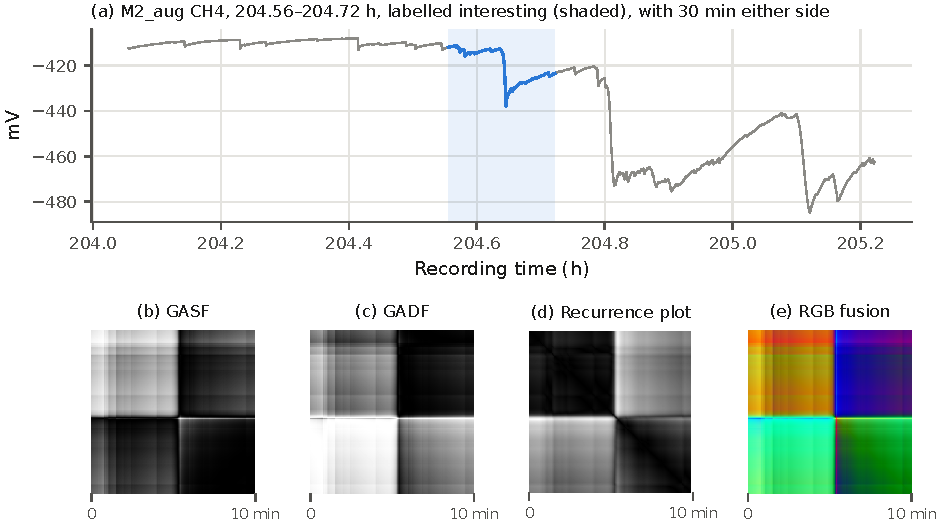
\includegraphics[width=\textwidth]{new/ch2_encodings.pdf}
\caption[{One 10-minute window and its four image encodings.}]{One 10-minute window and its four image encodings, the inputs of the CNN models. (a) A window of M2\_aug CH4 at 204.6 hours that was hand-labelled interesting (shaded), with 30 minutes of signal either side; it spans about 27\,mV. (b--e) The same 600 samples as a GASF, a GADF, a recurrence plot and the RGB fusion of the three, computed with the encoding functions the CNNs were trained with. Time runs along both axes of each image, so the sharp fall about halfway through the window splits every image into four blocks: pairs of moments both before the fall, both after it, or one on each side.}
\label{fig:encodings}
\end{figure}

\clearpage

\section*{From Chapter~\ref{ch:early}: early experimental work}

\begin{figure}[htbp]
\centering
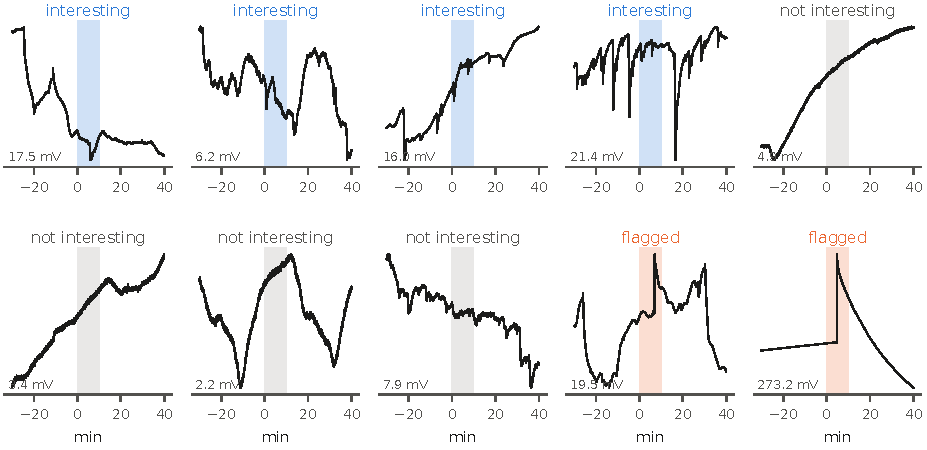
\includegraphics[width=\textwidth]{new/ch3_hand_labels.pdf}
\caption[{What the hand labels looked like.}]{What the hand labels looked like: ten of the 11,234 labelled 10-minute windows of M2\_aug (shaded), each in half an hour of context either side, with the peak-to-peak range of the panel. Four were labelled interesting, four not interesting and two flagged as artefacts.}
\label{fig:handlabels}
\end{figure}

\begin{figure}[htbp]
\centering
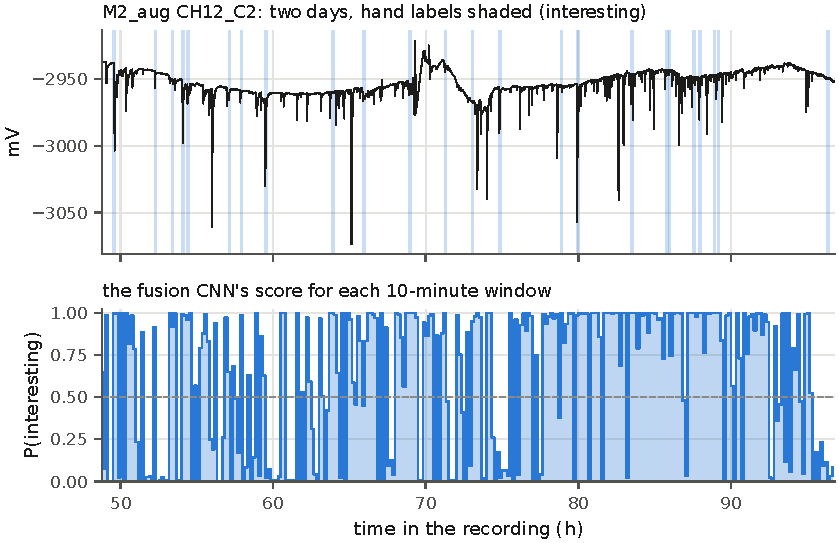
\includegraphics[width=\textwidth]{new/ch3_cnn_trace.pdf}
\caption[{What an early CNN's score looks like along a recording.}]{What an early CNN's score looks like along a recording: two days of one M2\_aug channel with the hand labels judged interesting shaded (top), and the fusion CNN's probability of ``interesting'' for each 10-minute window (bottom, from its stored sweep run). On this busy channel the CNN calls most windows interesting, far more than the hand labels do.}
\label{fig:cnnscoretrace}
\end{figure}

\begin{figure}[htbp]
\centering
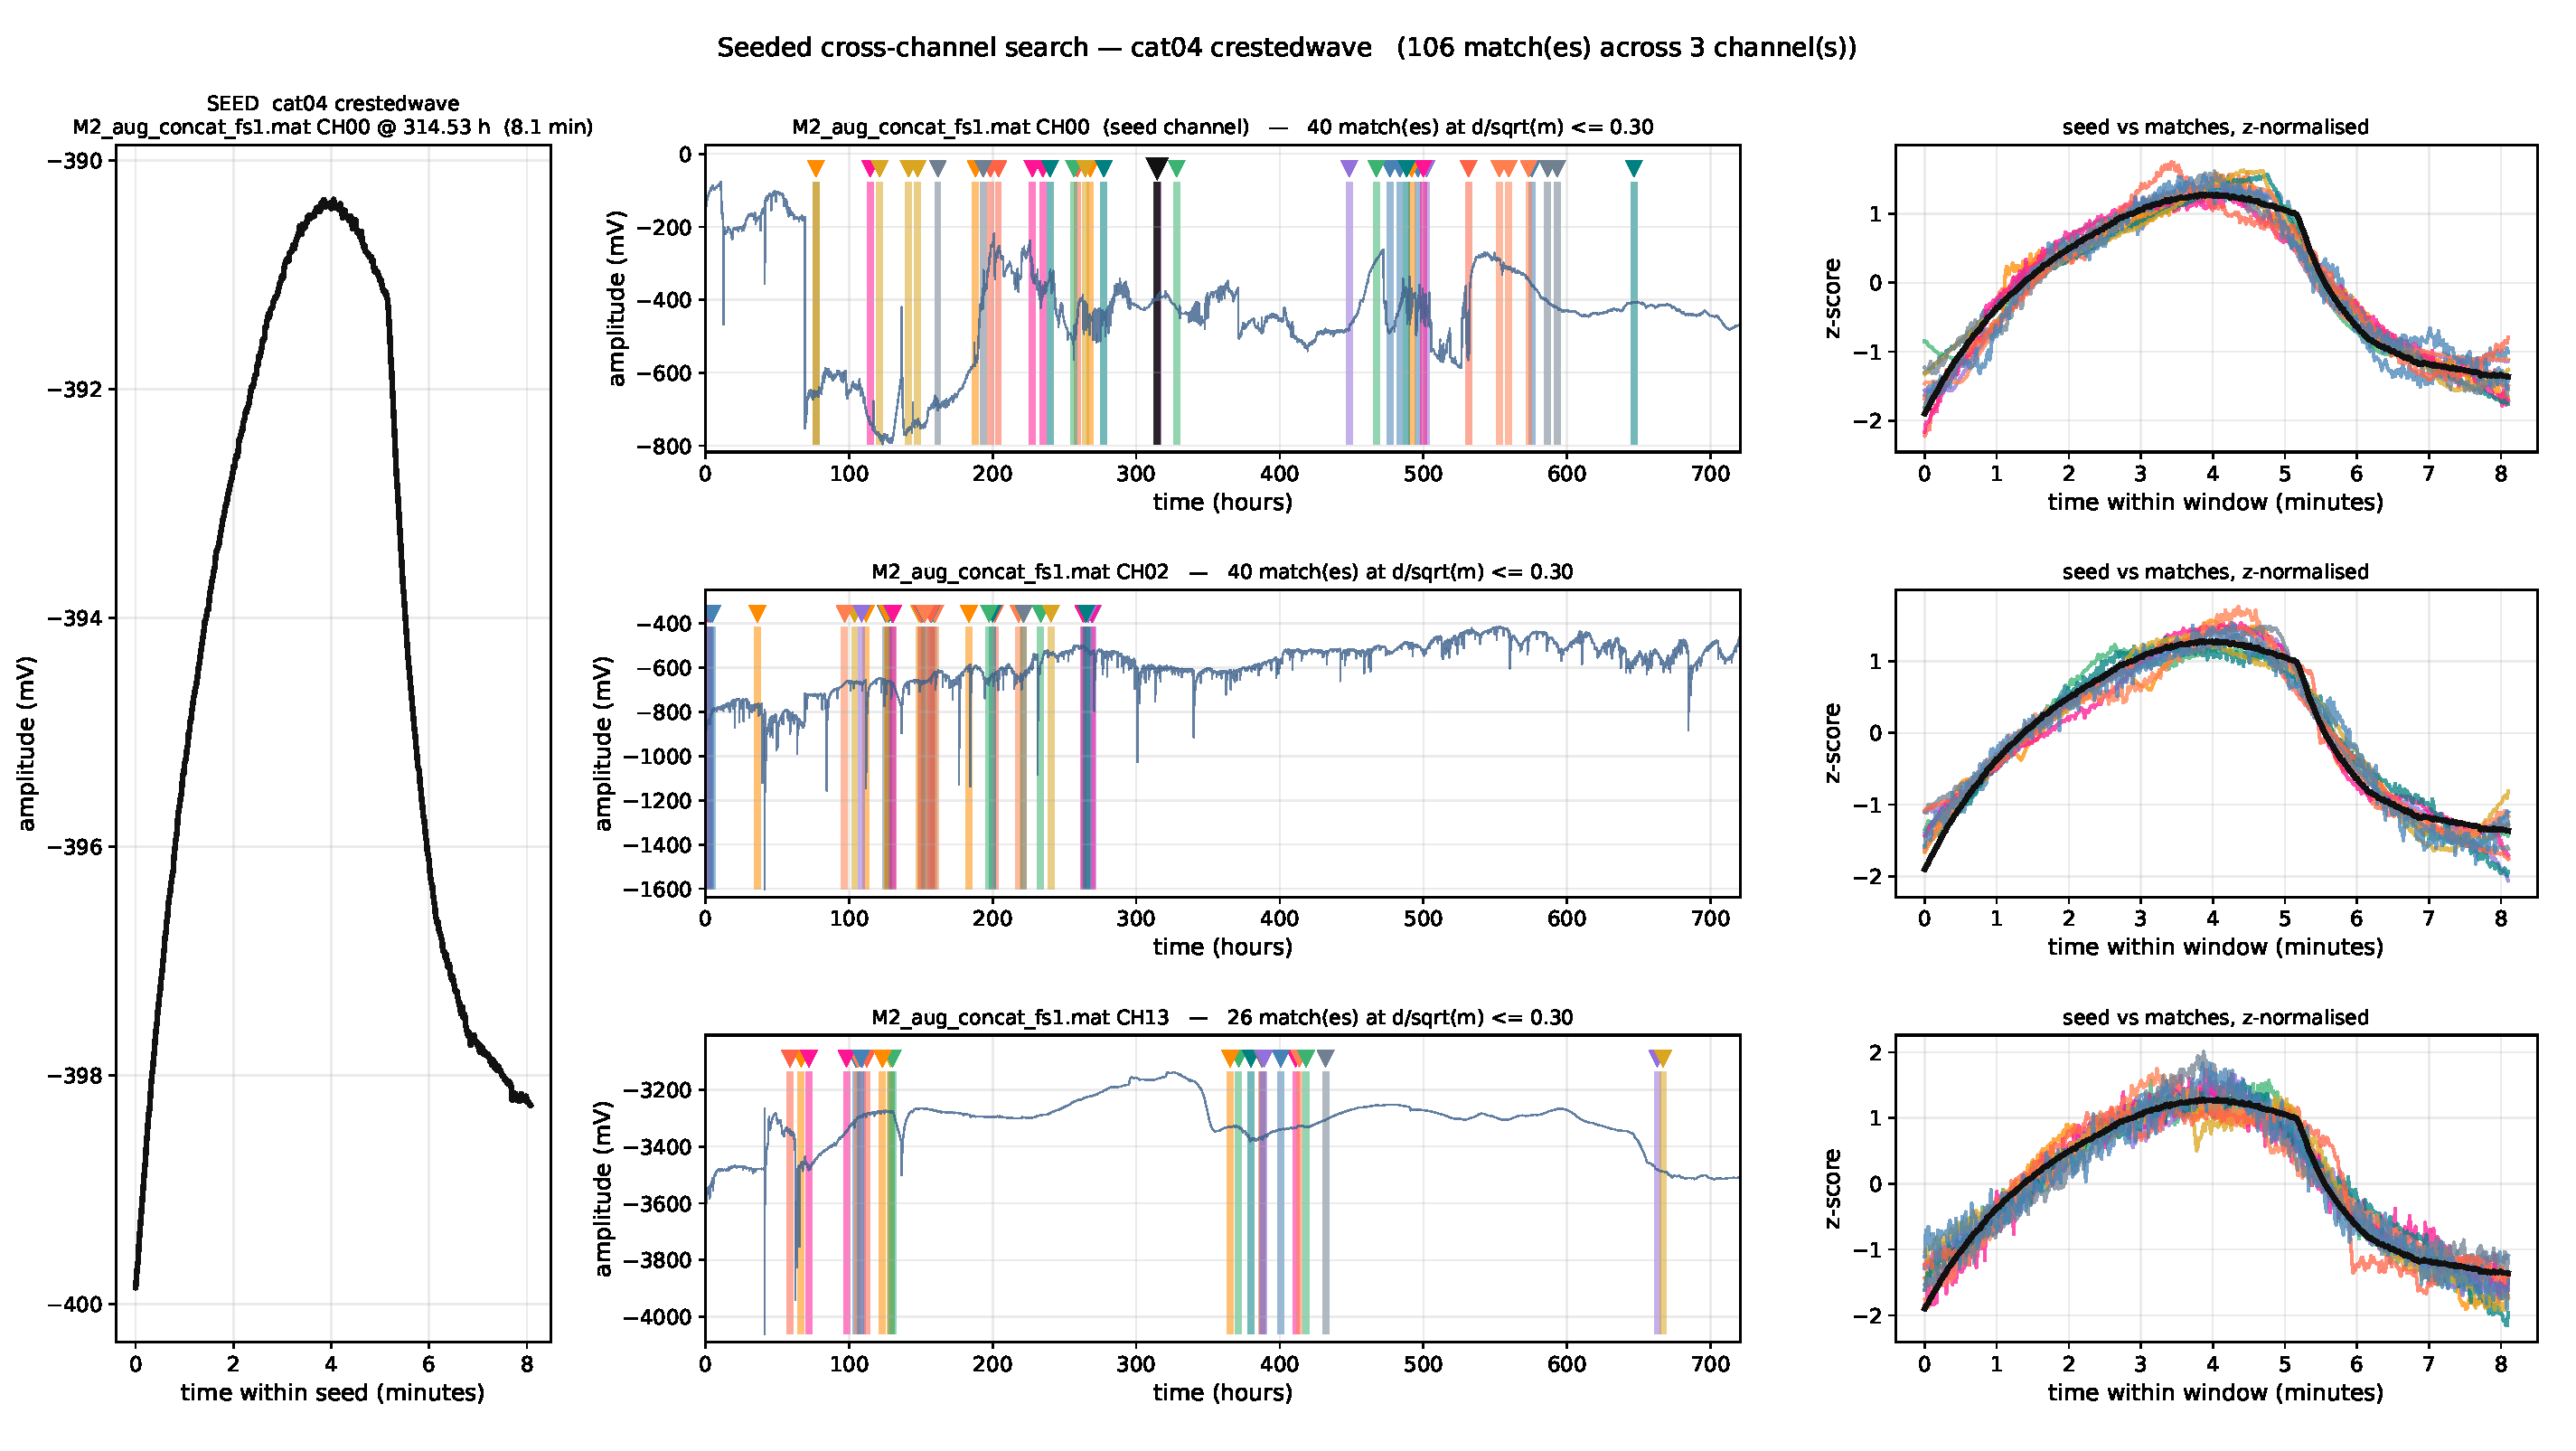
\includegraphics[width=\textwidth]{early/search_cat04_crestedwave.pdf}
\caption[{Seeded search across channels, from the early work.}]{Seeded search across channels, from the early work: one hand-catalogued ``crested wave'' on M2\_aug CH00 at 314.5\,h (left) used as a seed. Its matches at a z-normalised distance of at most 0.30 per $\sqrt{m}$ are marked along three channels of the 721-hour recording (middle; 106 in all), and overlaid z-normalised on the seed (right).}
\label{fig:mpseed}
\end{figure}

\begin{figure}[htbp]
\centering
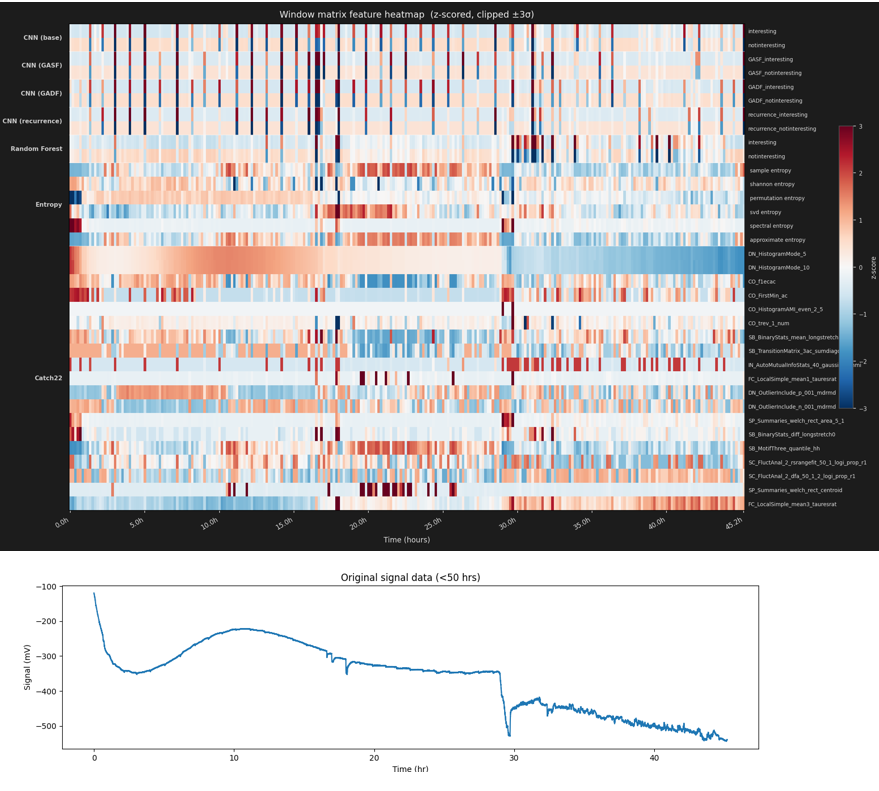
\includegraphics[width=\textwidth]{plan/window_matrix.png}
\caption[{An early Window Matrix, as exported at the time.}]{An early Window Matrix, as exported at the time (dark theme), over the first 45 hours of a primary recording. Each row is one feature, grouped as CNN outputs, random-forest outputs, entropy measures and catch22 features, z-scored and clipped at $\pm3\sigma$; each column is one 10-minute window, and the signal for the same hours is drawn beneath. Many features change together where the signal changes, for example at the sharp fall near 29 hours. Because the matrix has one row per window and no alignment to individual samples, it could describe windows but not mark where an event began or ended (Section~\ref{sec:representation}).}
\label{fig:windowmatrix}
\end{figure}

\begin{figure}[htbp]
\centering
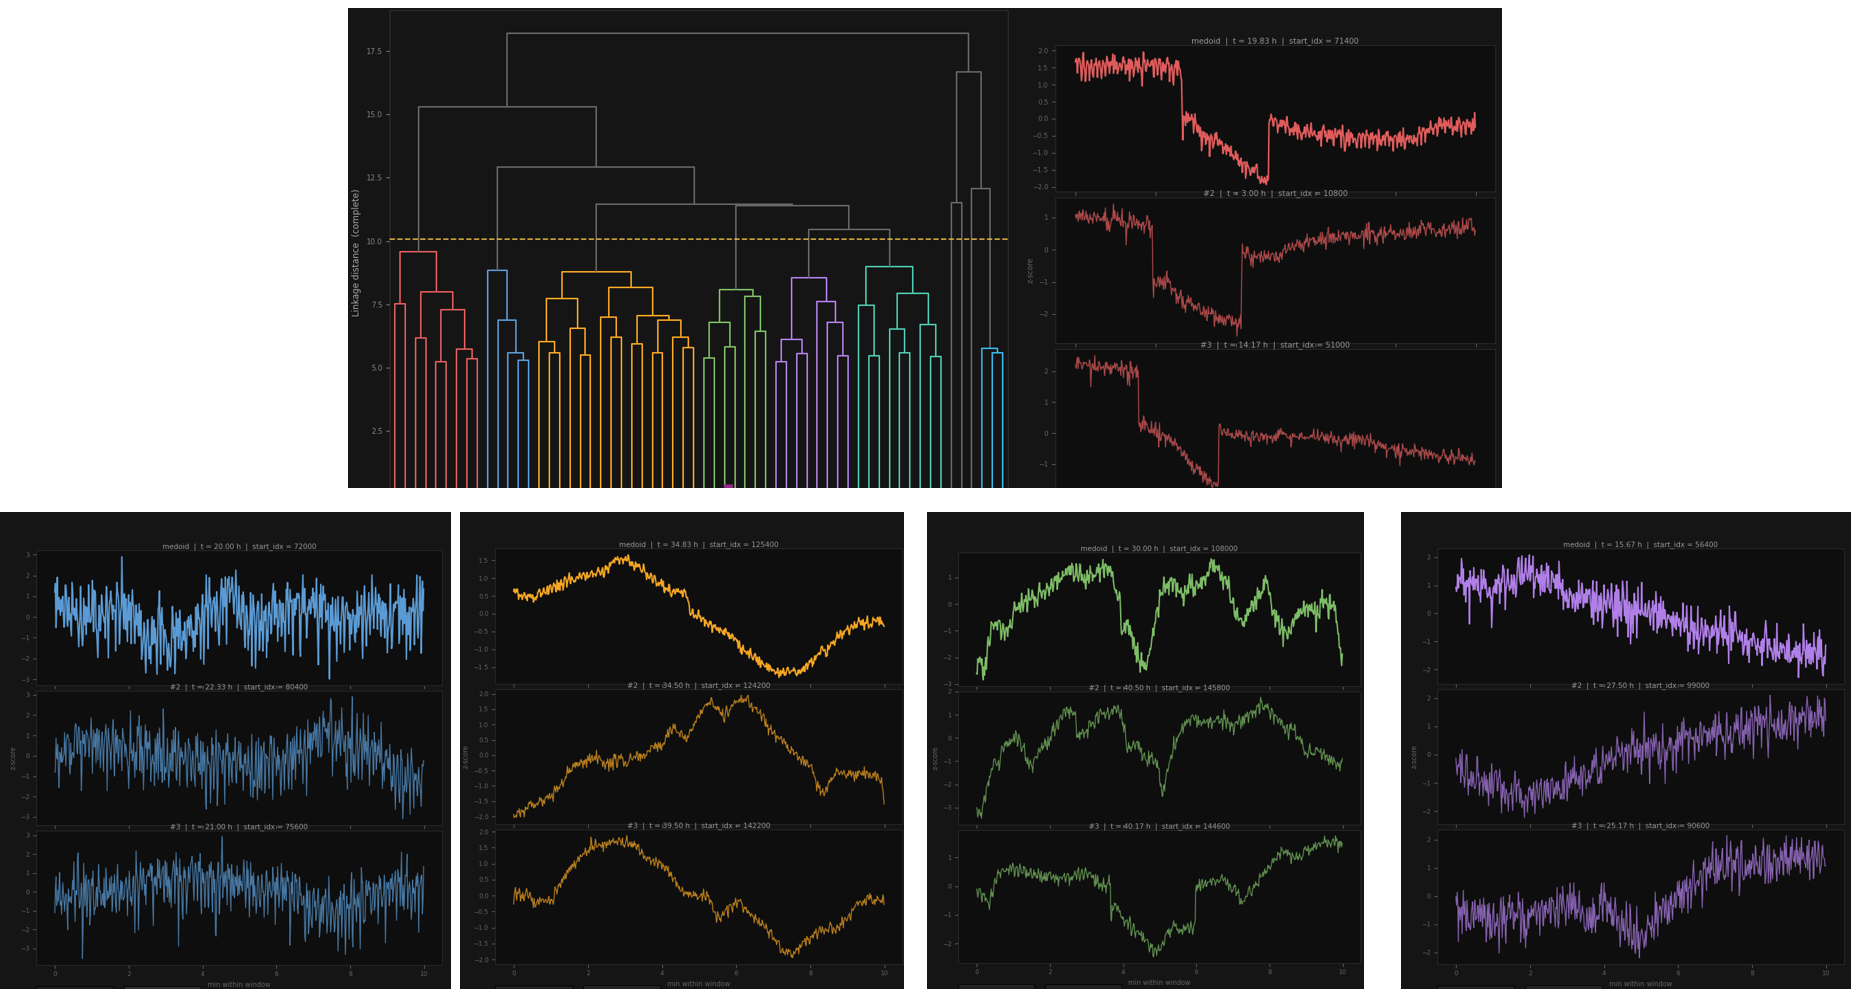
\includegraphics[width=\textwidth]{plan/dendrogram_plan_clean.png}
\caption[{An early dendrogram of 10-minute windows (May 2026).}]{An early dendrogram of 10-minute windows from the May 2026 clustering experiments, as exported at the time: complete linkage on z-normalised Euclidean distance, with the dashed line marking one possible cut. Each coloured cluster is shown by its medoid window and two further members (red, top right; the other four below). The clusters do separate step-like falls, noisy flat stretches, slow waves and drifts, but moving the cut merged or split them, and no number of clusters settled as the right one.}
\label{fig:dendroplan}
\end{figure}

\begin{figure}[htbp]
\centering
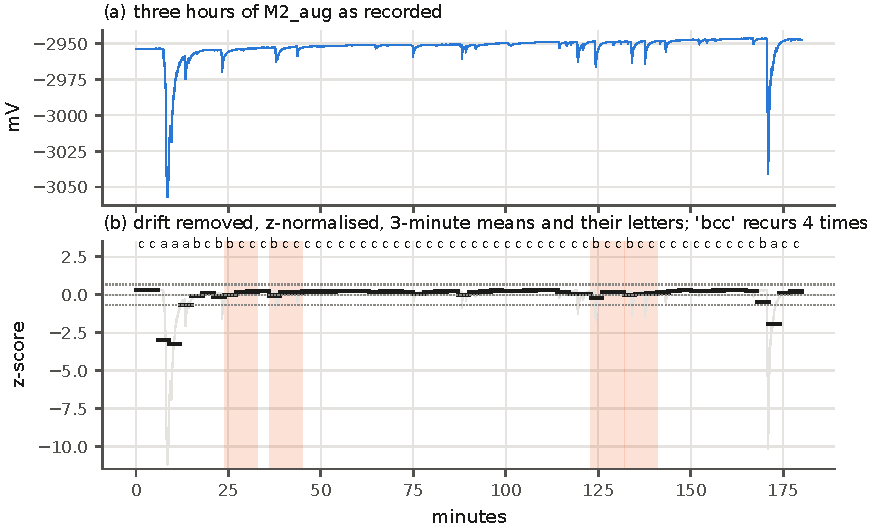
\includegraphics[width=\textwidth]{new/ch3_sax.pdf}
\caption[{SAX on a real trace.}]{SAX on a real trace. (a) Three hours of M2\_aug. (b) The same, with the slow drift removed and z-normalised, reduced to 3-minute means (bars), each coded as one of four letters by the dotted breakpoints; the most frequent mixed three-letter word is shaded. A few deep falls stretch the scale, so almost every other window becomes the same letter: the problem the early SAX experiments met, and one reason the tool's symbolic route normalises locally.}
\label{fig:sax}
\end{figure}

\begin{figure}[htbp]
\centering
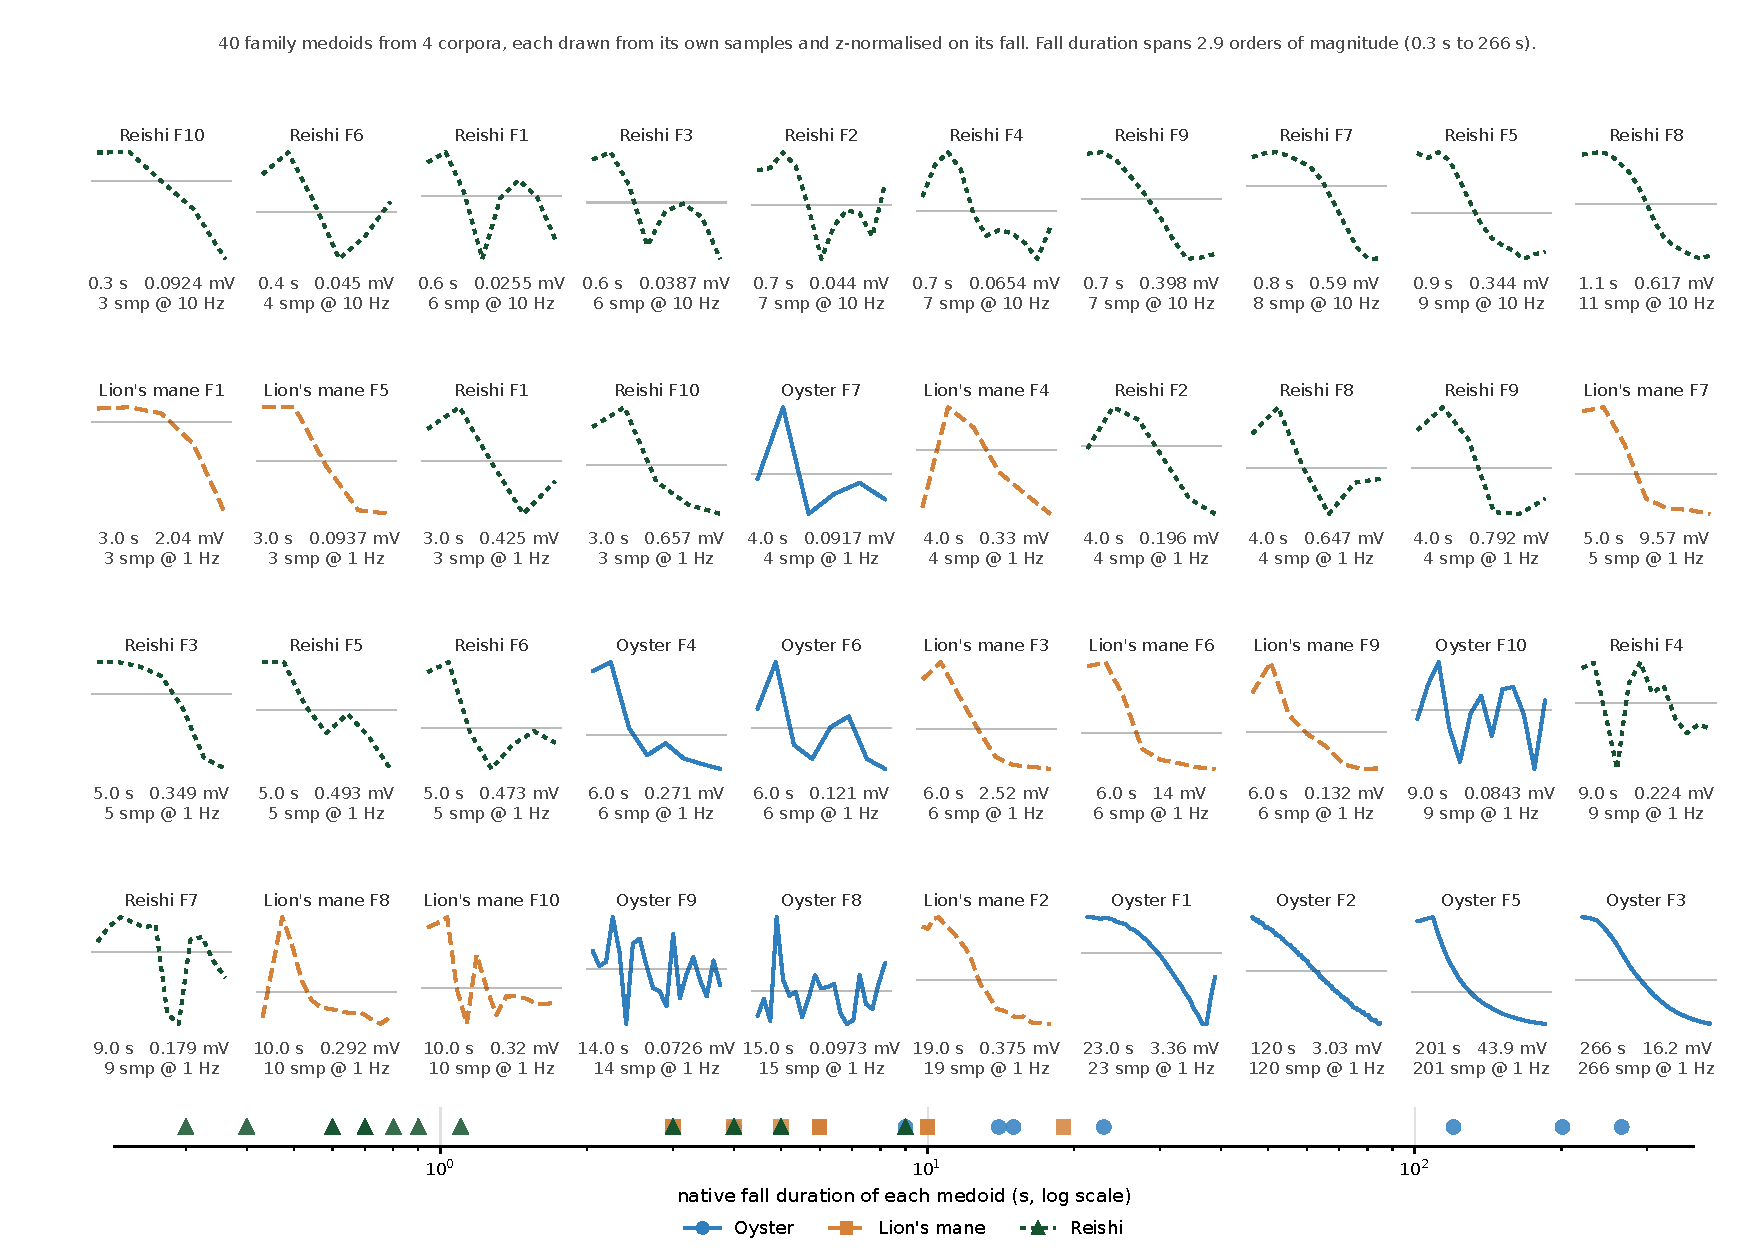
\includegraphics[width=\textwidth]{drop_motifs/ATLAS_shapes.pdf}
\caption[{Forty family medoids from the drop-motif study's four corpora.}]{Forty family medoids from the drop-motif study's four corpora (oyster, the lion's mane excerpt, and reishi at its native 10\,Hz and resampled to 1\,Hz), placed by native fall duration: 0.3--266\,s, 2.9 orders of magnitude. Each medoid is drawn normalised by its own fall. The shortest are built from only a handful of samples (3--6), so at that end the drawn shape mostly reflects the sampling rate rather than the waveform, which is the problem Figure~\ref{fig:speciesres} measures.}
\label{fig:atlas}
\end{figure}

\begin{figure}[htbp]
\centering
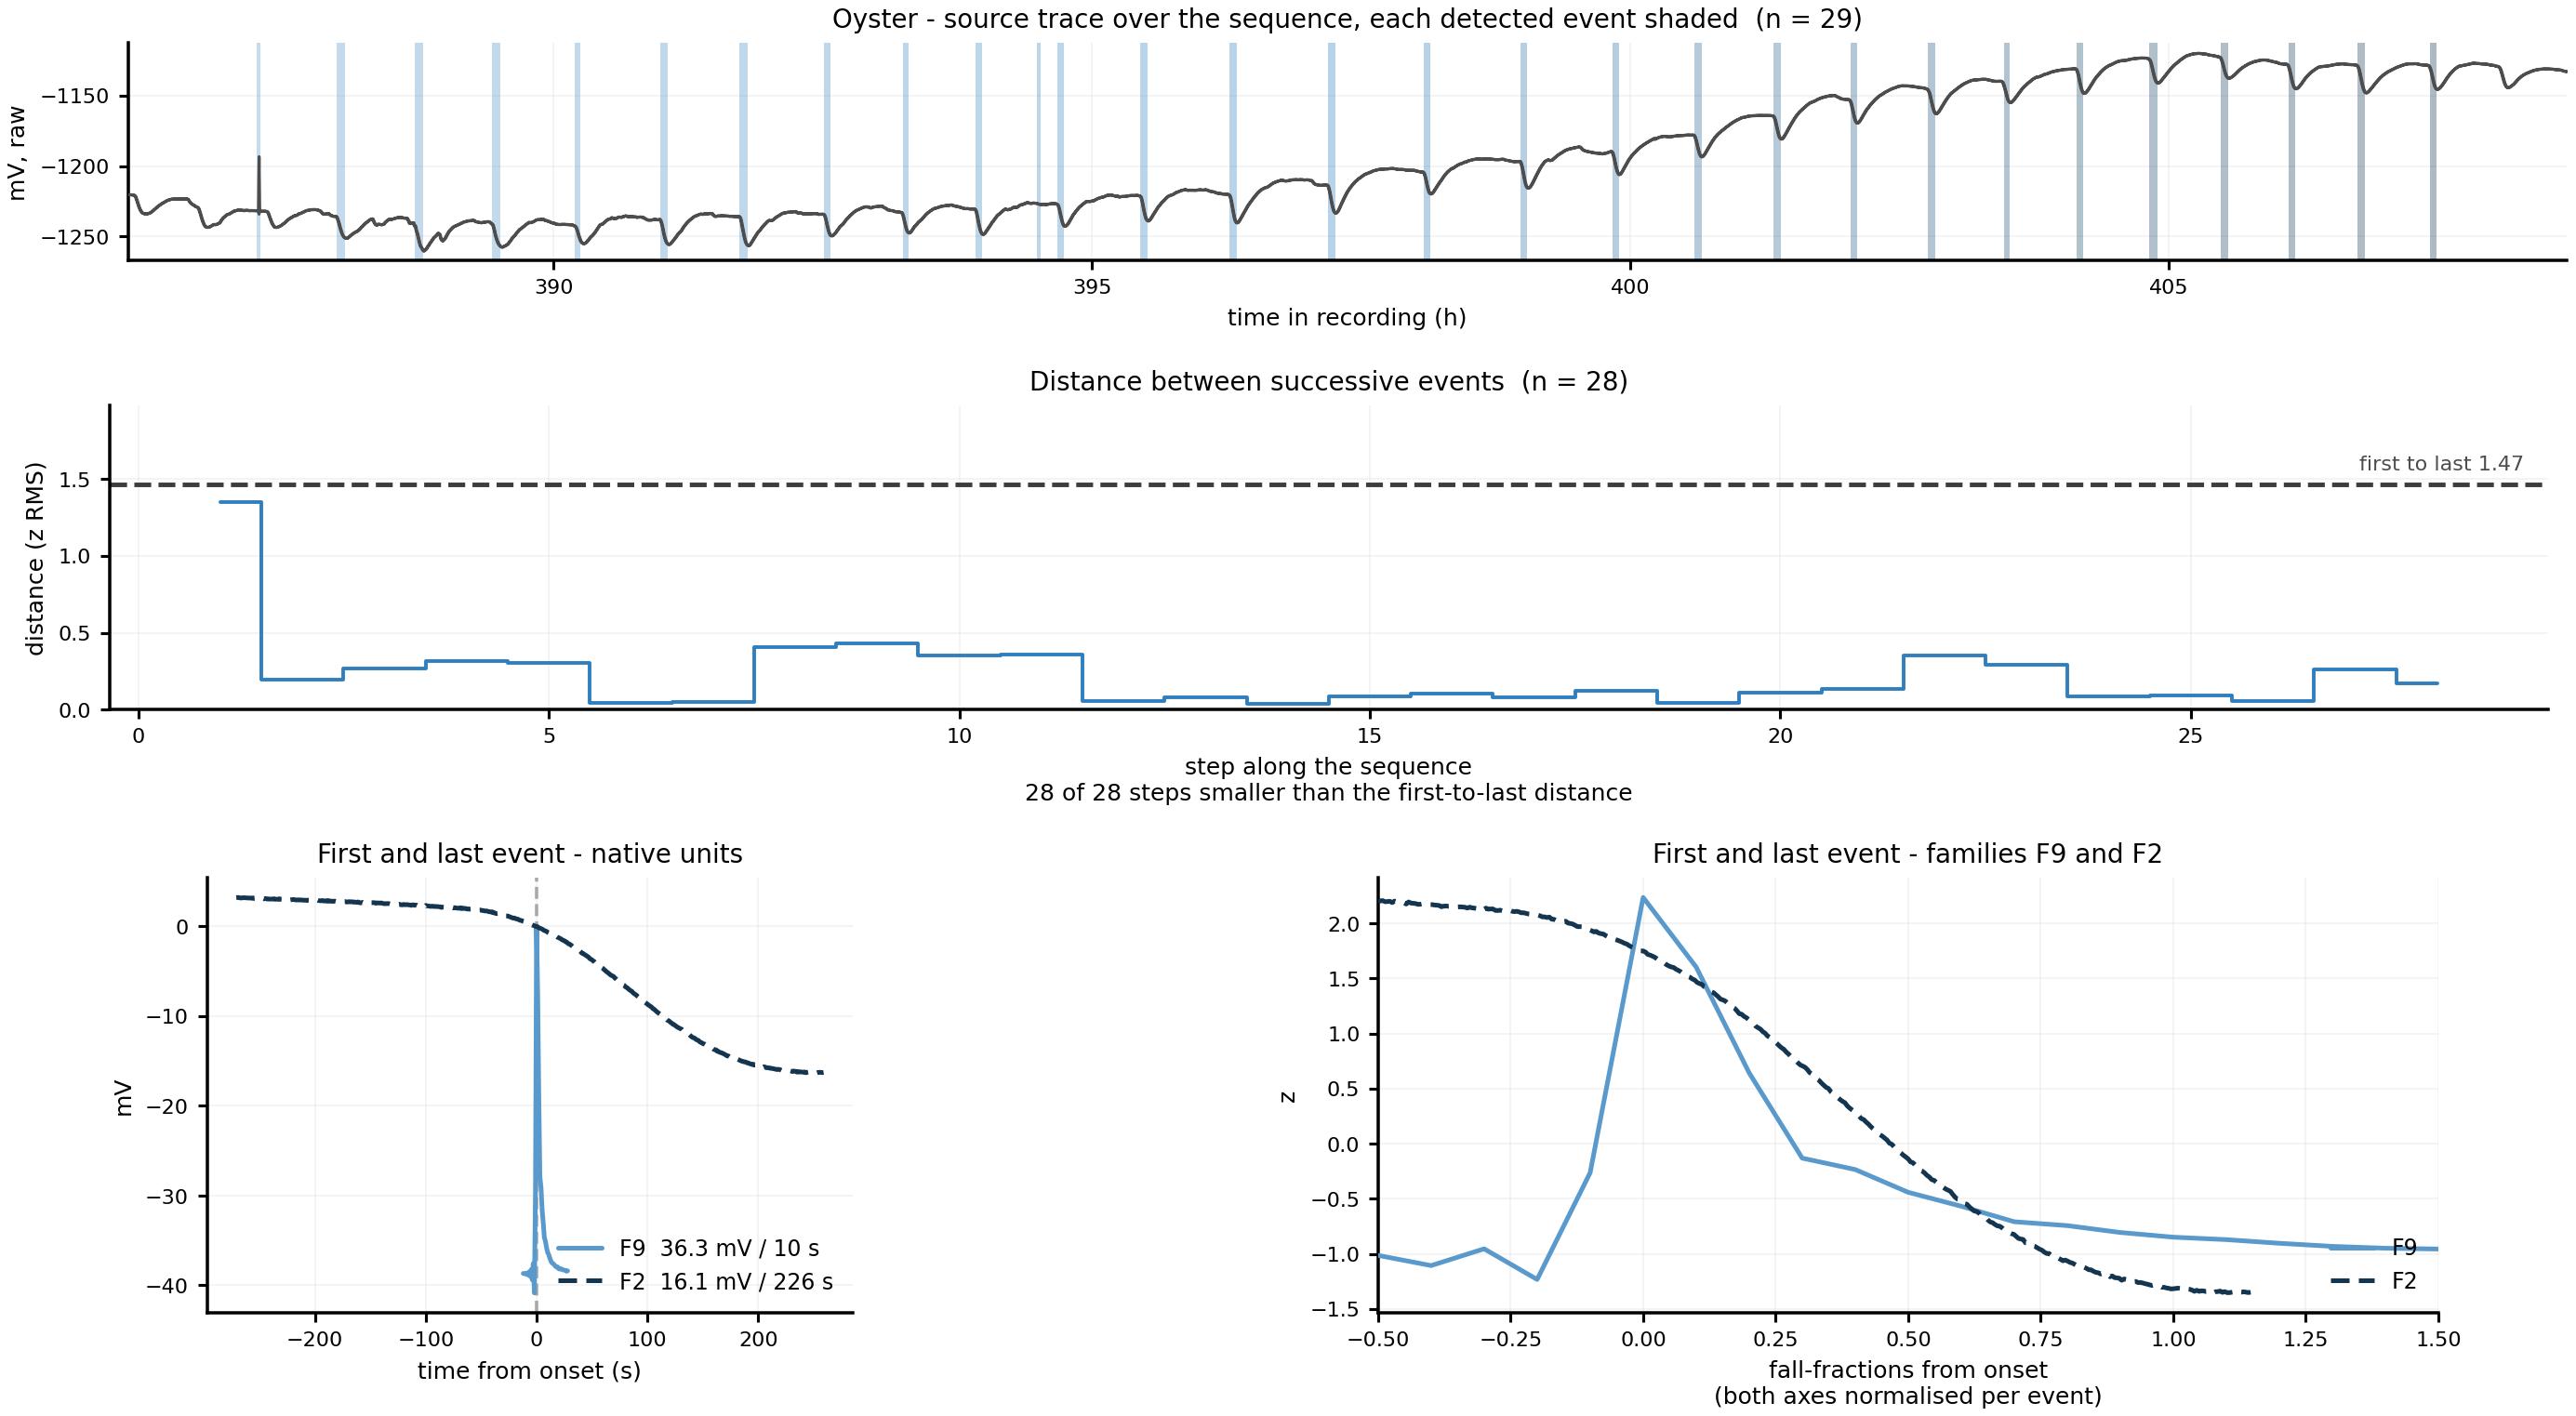
\includegraphics[width=\textwidth]{drop_motifs/S3_1_sequence_morph_short.png}
\caption[{A drop sequence from the drop-motif study (M2\_aug CH6\_B1, 387--408\,h).}]{A drop sequence from the drop-motif study: M2\_aug CH6\_B1 (stored as channel 5), 387--408 hours. Top: the trace, with each of its 29 detected drops shaded; the drops repeat about every 40 minutes while the baseline climbs by about 100\,mV. Middle: the shape distance from each drop to the next, against the distance from the first drop to the last (dashed). All 28 steps are smaller than that, which the study read as a gradual morph, but the first step accounts for almost all of the change: the first event is a sharp 36\,mV spike, and the drops after it change little from one to the next. Bottom: the first and last events in native units and normalised by their fall. Chapter~\ref{ch:roundb} (B2) tests sequences like this against shuffled orders and finds persistence rather than a steady morph.}
\label{fig:sequence}
\end{figure}

\begin{figure}[htbp]
\centering
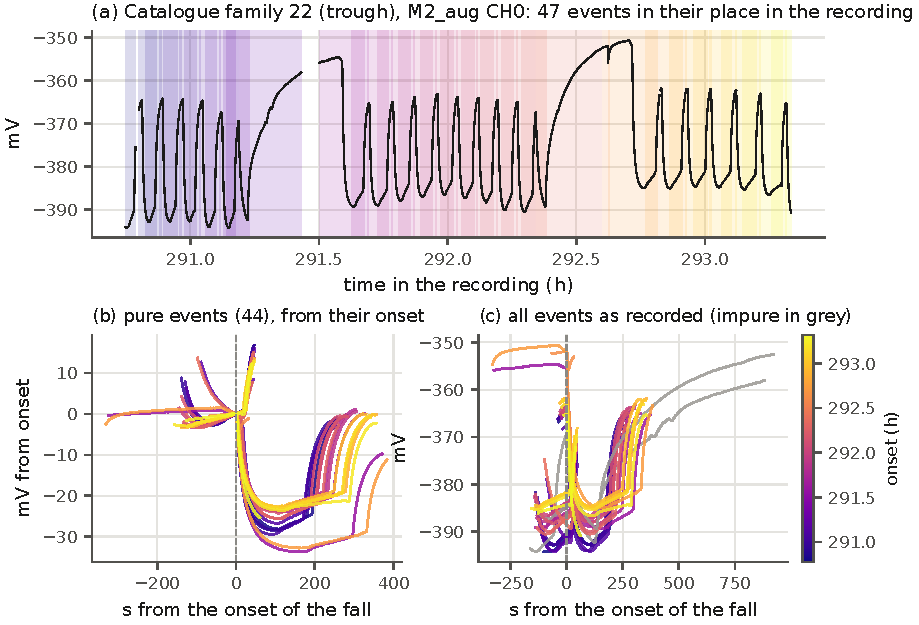
\includegraphics[width=\textwidth]{new/ch3_drop_family.pdf}
\caption[{One hand-catalogued drop family from the drop-motif study.}]{One hand-catalogued drop family from the drop-motif study: catalogue family 22, troughs on M2\_aug CH1\_A1 (stored as channel 0) near 291--293\,h. (a) Its 47 events (two detection passes, 24 coarse and 23 fine) in their place in the recording, each window shaded by its onset time; the short break near 291.45\,h is a gap in the recording. (b) The 44 pure events (one fall per window) drawn from the onset of their fall, baseline removed and amplitude not scaled: a fall of 20--30\,mV, a trough lasting about three minutes, then a fast return. (c) Every event as recorded, with the three impure ones in grey. The same fall, trough and return repeats every few minutes for two and a half hours, at two time scales.}
\label{fig:droptrio}
\end{figure}

\clearpage

\section*{From Chapter~\ref{ch:pipeline}: \tool{}}

\begin{table}[htbp]
\caption[{Registered analysis blocks by stage (59 in all).}]{Registered analysis blocks by stage (59 in all). The full list is in Appendix~\ref{app:blocks}.}
\label{tab:blockstages}
\small
\begin{tabularx}{\textwidth}{p{2.6cm} r X}
\toprule
\textbf{Stage} & \textbf{Blocks} & \textbf{Examples}\\
\midrule
Preprocessing & 14 & detrend, band-pass, BEADS baseline, invert, wavelet bands, surrogate, window matrix\\
Detection & 24 & drop detector, matrix profile, seed matches, OASIS deconvolution, Dehshibi spikes, FLUSS, change points, SAX/dSAX, symbol search, wavelet scattering\\
Catalogue & 16 & Gramian encodings, CNN window scores, MiniRocket, shape families, clustering, manual labels\\
Interrogation & 5 & event shape, intervals, trains, cycle shapes, event families\\
\bottomrule
\end{tabularx}
\end{table}

\begin{table}[htbp]
\caption[{Planned scope exclusions against the software as built.}]{Planned scope exclusions (August 2026) against the software as built (October 2026).}
\label{tab:scope}
\small
\begin{tabularx}{\textwidth}{p{4.2cm} p{2.2cm} X}
\toprule
\textbf{Planned exclusion} & \textbf{Status} & \textbf{As built}\\
\midrule
Multivariate analysis & partly built & Cross-channel lag, correlation and three-bin classification, and an Explore cross-channel page; no multivariate models.\\
Data import robustness & built & Registration with checks, excerpt detection, unit and rate inference, a Settings import page.\\
An open plugin architecture & not built & The block contract makes a new block easy to add; there is no third-party registry.\\
A drag-and-drop node canvas & not built & Chains are a linear ribbon of typed blocks.\\
Rendered report generation & built & HTML, Markdown and figure reports per run.\\
Cross-domain corpora & not built & No non-fungal control; cross-species fungal data was added instead.\\
A supported software release & partly & A 342-page user manual; not packaged or supported.\\
Biological interpretation & excluded & Unchanged (Section~\ref{sec:position}).\\
\bottomrule
\end{tabularx}
\end{table}

\clearpage

\section*{From Chapter~\ref{ch:method}: methodology}

\begin{table}[htbp]
\caption[Classification of cross-channel matches]{Classification of cross-channel co-occurrences, as implemented in \texttt{Working/cross\_channel.py} and the detector census of \texttt{Working/cross\_census.py} (Chapter~\ref{ch:roundb}). Two onsets co-occur when they fall within 50\,s of each other. Bin edges are editable in Settings.}
\label{tab:crosschannel}
\begin{center}
\small
\begin{tabular}{p{3.2cm} p{4.6cm} p{5.6cm}}
\toprule
\textbf{Bin} & \textbf{Signature} & \textbf{Interpretation}\\
\midrule
Artifact (common mode) & $|\text{lag}|\le1$\,s and $|r|\ge0.98$, any packs & A copy of one waveform at the same instant, most likely through the shared ground; flagged for a human, excluded from recurrence counts only once confirmed\\
\addlinespace
Propagation & Same pack, 1--50\,s lag and $|r|\ge0.5$ & A single event travelling through one network; counted once\\
\addlinespace
Shared driver & Different packs, not a copy & Separate cultures reacting to one outside influence (environment or recording setup); never counted as propagation\\
\addlinespace
Independent recurrence & Same pack, anything else that beats chance & Genuine recurrence; counted once per instance\\
\bottomrule
\end{tabular}
\end{center}
\end{table}

\clearpage

\section*{From Chapter~\ref{ch:rq1}: detectors}

\begin{table}[htbp]
\caption[{Six precise settings on M2\_aug against 20 phase-randomised draws.}]{Six precise variants on M2\_aug against 20 phase-randomised draws per channel (16 channels each). ``Beat all'' and ``below all'': channels whose real count lies above or below every one of its 20 draws; chance expects 0.8 of 16. Precision is from the M2\_aug blind detector panel.}
\label{tab:surr20}
\footnotesize
\centering
\setlength{\tabcolsep}{4pt}
\begin{tabular}{lcccccc}
\toprule
\textbf{Variant} & \textbf{Precision} & \textbf{Beat all} & \textbf{Below all} & \textbf{Ratio, 20} & \textbf{Ratio, 1} & \textbf{BH}\\
\midrule
drop v1 & 0.94 & 16/16 & 0/16 & 23.4 & 22.6 & pass\\
CNN GADF, 10 min & 0.97 & 16/16 & 0/16 & 6.5 & 6.5 & pass\\
CNN recurrence, 10 min & 0.96 & 14/16 & 1/16 & 2.7 & 2.6 & pass\\
drop v5, same fraction 0.7 & 0.81 & 14/16 & 2/16 & 2.2 & 2.2 & pass\\
drop v1, slope $\sigma$ 4 & 0.99 & 3/16 & 12/16 & 0.58 & 0.60 & --\\
wavelet-encoded, level 5 & 0.92 & 0/16 & 16/16 & 0.075 & 0.075 & --\\
\bottomrule
\end{tabular}
\end{table}

\begin{figure}[htbp]
\centering
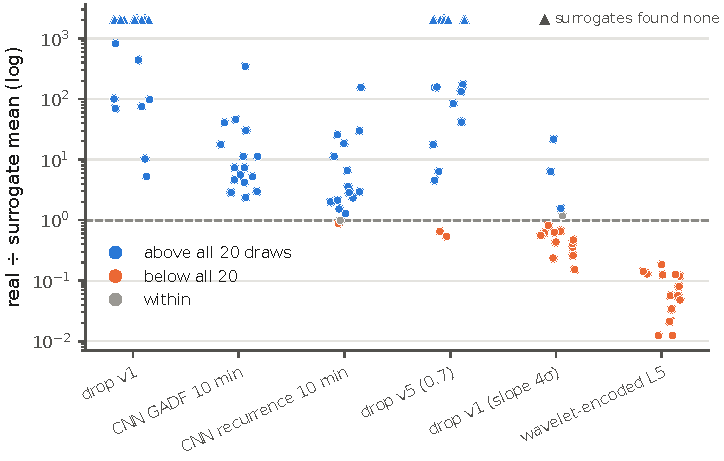
\includegraphics[width=0.85\textwidth]{new/ch6_surr20.pdf}
\caption[{Six detector settings on M2\_aug's 16 channels.}]{Six detector settings on M2\_aug's 16 channels, each channel's real detection count over the mean of 20 surrogate draws (log scale). Blue: above every draw; orange: below every draw; grey: within. Triangles at the top mark channels whose 20 draws found nothing.}
\label{fig:surr20}
\end{figure}

\begin{table}[htbp]
\centering
\caption[{Selected detector settings against the original M2\_aug window labels.}]{Selected detector settings against the original M2\_aug window labels. Each setting ran on all 16 channels, covering 2,333 interesting and 8,773 uninteresting windows. A touch is any overlap. Lift is the interesting-window touch rate divided by the uninteresting-window touch rate, calculated before rounding. The full comparison is in Appendix~\ref{app:windowtouch}.}
\label{tab:windowtouch}
\small
\setlength{\tabcolsep}{4pt}
\begin{tabularx}{\textwidth}{@{}>{\raggedright\arraybackslash}X r r r@{}}
\toprule
\textbf{Detector setting} & \makecell{\textbf{Interesting}\\\textbf{touched (\%)}} & \makecell{\textbf{Uninteresting}\\\textbf{touched (\%)}} & \textbf{Lift}\\
\midrule
OASIS, threshold 3 & 90.6 & 65.6 & 1.4\\
OASIS, threshold 5 & 48.7 & 11.2 & 4.4\\
Signal threshold, $-2$\,mV & 51.2 & 5.3 & 9.7\\
Signal threshold, $-10$\,mV & 12.4 & 0.6 & 21.3\\
Drop detector v1, default & 7.0 & 1.3 & 5.3\\
\bottomrule
\end{tabularx}
\end{table}

\begin{figure}[htbp]
\centering
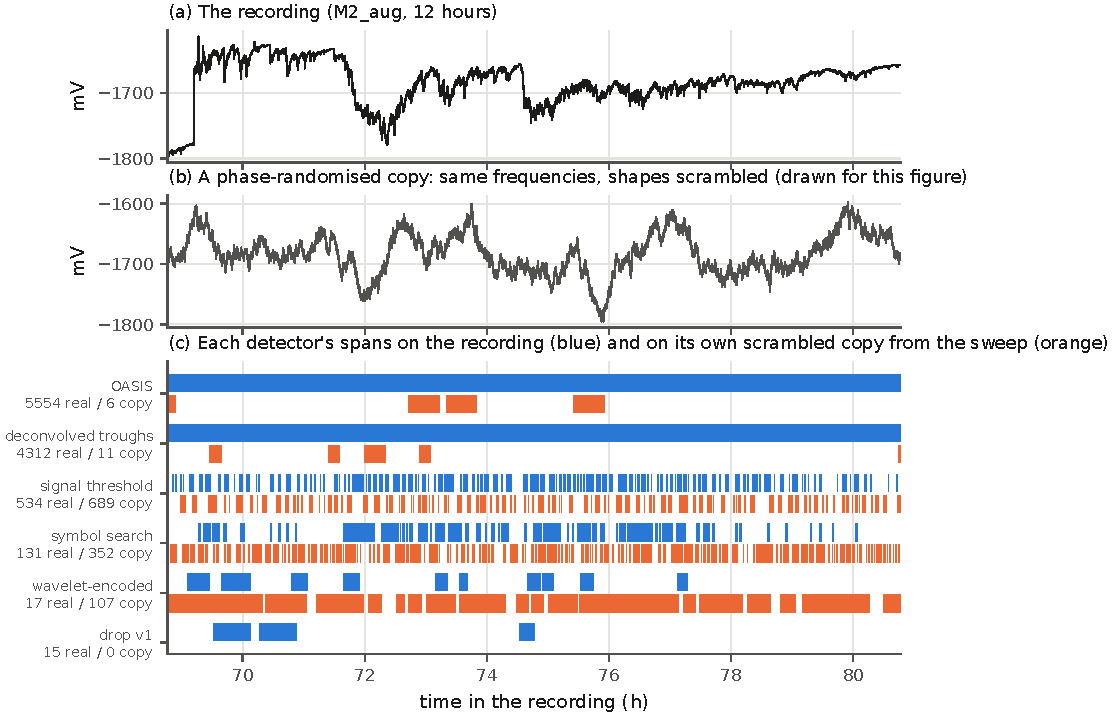
\includegraphics[width=\textwidth]{new/ch6_real_vs_surrogate.pdf}
\caption[{The surrogate test in a 12-hour excerpt of M2\_aug.}]{The surrogate test in a 12-hour excerpt of M2\_aug. (a) The recorded voltage. (b) Each row shows the detections from one setting of the sweep, run on the recording (upper blue strip) and on its phase-randomised copy (lower orange strip). The numbers count spans that intersect the excerpt, including overlaps. Changing the OASIS threshold reduces the number of proposals in this window by a factor of ten. Wavelet-encoded level~3 fires more often on the copy, while default drop v1 fires only on the recording.}
\label{fig:realvssurr}
\end{figure}

\begin{figure}[htbp]
\centering
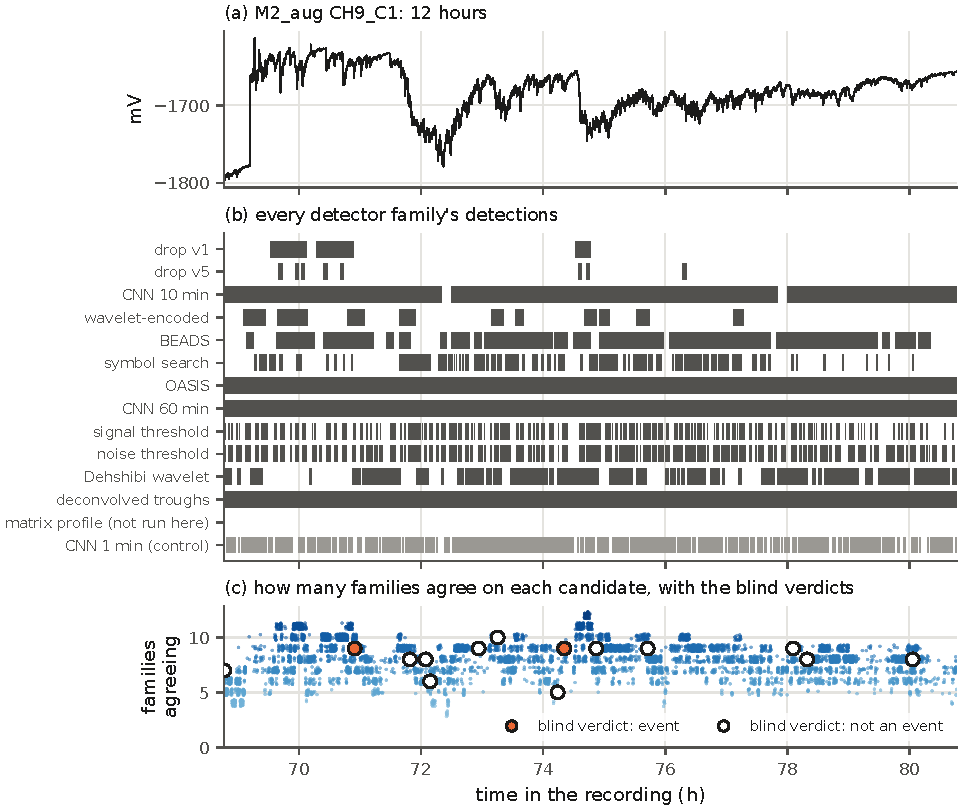
\includegraphics[width=\textwidth]{new/ch6_agreement_excerpt.pdf}
\caption[{What agreement looks like, on 12 hours of one M2\_aug channel.}]{What agreement looks like, on 12 hours of one M2\_aug channel. (a) The signal. (b) Every detector family's detections: the loose families (OASIS, the deconvolved troughs, the 60-minute CNN) cover almost all of it, while the choosy ones (drop v1 and v5) mark only a few stretches around the sharpest changes; the matrix-profile threshold was not run on this channel. (c) The candidate events of up to 30 minutes, by how many families agree on them, and the blind verdicts given in this window. The two candidates judged to be events sit where agreement is highest, near the sharp changes at about 71 and 74.5 hours, while most candidates at seven to ten agreeing families were judged not to be events. One window holds only a handful of verdicts; the ladder (Figure~\ref{fig:ladder}) is the same picture over all 1,864 answered verdicts (1,959 reviewed, less 95 unsure).}
\label{fig:agreementexcerpt}
\end{figure}

\clearpage

\section*{From Chapter~\ref{ch:rq2}: seeds}

\begin{table}[htbp]
\caption[{Matches per channel for each seed in M2\_aug.}]{Matches per channel for each seed in M2\_aug, at the common thresholds of Table~\ref{tab:seeds}. Zero means that the channel was searched but no match passed the threshold; a dash means that the channel was not searched. These are search returns, including the seed's own location; they are not counts of reviewed events.}
\label{tab:seedchannels}
\small
\centering
\begin{tabularx}{\textwidth}{@{}Xrrrr@{}}
\toprule
\textbf{Channel} & \makecell[r]{\textbf{Short dip}\\\textbf{105\,s}} & \makecell[r]{\textbf{Long dip}\\\textbf{816\,s}} & \makecell[r]{\textbf{Spike}\\\textbf{148\,s}} & \makecell[r]{\textbf{Drop}\\\textbf{377\,s}}\\
\midrule
CH1\_A1 & -- & 14 & 16 & 54\\
CH2\_A1 & 14 & 20 & 0 & 111\\
CH3\_A2 & -- & 5 & 0 & 7\\
CH4\_A2 & -- & 19 & 0 & 66\\
CH5\_B1 & -- & 6 & 0 & 17\\
CH6\_B1 & 12 & 6 & 0 & 1\\
CH7\_B2 & 38 & 6 & 0 & 3\\
CH8\_B2 & -- & 4 & 0 & 14\\
CH9\_C1 & -- & 6 & 0 & 18\\
CH10\_C1 & -- & 7 & 0 & 5\\
CH11\_C2 & -- & 4 & 0 & 17\\
CH12\_C2 & -- & 2 & 0 & 2\\
CH13\_D1 & -- & 3 & 0 & 8\\
CH14\_D1 & -- & 4 & 0 & 2\\
CH15\_D2 & -- & 12 & 0 & 13\\
CH16\_D2 & -- & 6 & 0 & 34\\
\midrule
Total & 64 & 124 & 16 & 372\\
\bottomrule
\end{tabularx}
\end{table}

\begin{figure}[htbp]
\centering
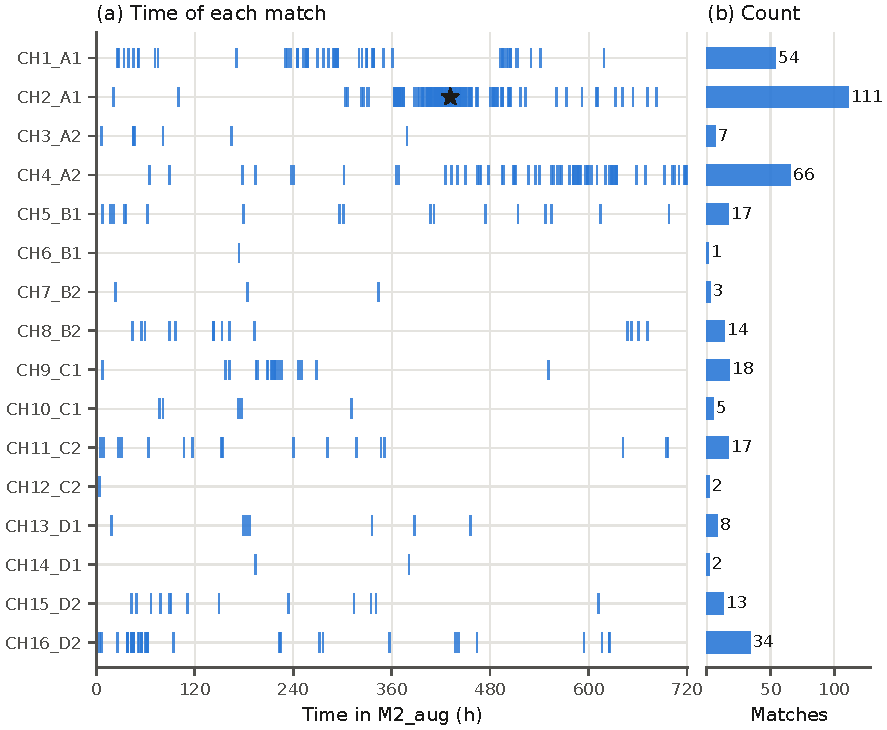
\includegraphics[width=\textwidth]{new/ch7_drop_distribution.pdf}
\caption[{Where and when the 372 drop-seed matches occur in M2\_aug.}]{Distribution of all 372 drop-seed matches passing the common shape-distance threshold of 2.208 in M2\_aug. Left: each mark is a match onset over the 721 hours searched on every channel; the star marks the original seed. Right: totals for the same channels. These are the full search returns; the 100 matches judged in the blind panel were a subset.}
\label{fig:dropdistribution}
\end{figure}

\clearpage

\section*{From Chapter~\ref{ch:rq3}: classifiers}

\begin{table}[htbp]
\centering
\caption[{Initial random forests trained on manual and cluster-derived labels.}]{Initial random forests trained on manual and cluster-derived labels (run 79, M2\_aug, ten-minute windows). Macro F1 with 95\,\% bootstrap intervals; shuffle columns give mean scores after 200 training-label permutations and refits.}
\label{tab:forests}
\small
\begin{tabularx}{\textwidth}{@{}Xrccc@{}}
\toprule
\textbf{Test} & \textbf{$n$} & \textbf{Manual (A)} & \textbf{Cluster (B)} & \textbf{Null A/B}\\
\midrule
Unseen channels & 2,530 & 0.793 [0.764--0.819] & 0.635 [0.594--0.674] & 0.428/0.427\\
Later block & 1,549 & 0.884 [0.798--0.922] & 0.607 [0.524--0.662] & 0.480/0.477\\
\bottomrule
\end{tabularx}
\end{table}

\begin{table}[htbp]
\centering
\caption[{Manual forest A and seven-cluster forest B2 on blind ten-minute windows.}]{Manual forest A and revised seven-cluster forest B2 on the same blind ten-minute windows. The no-earlier-label subset excludes overlap with earlier labelled spans; M2\_concat is a separate recording. These are overlapping subsets, not additional independent tests. Precision and recall refer to the interesting class.}
\label{tab:forestblind}
\small
\begin{tabularx}{\textwidth}{@{}Xlrrrr@{}}
\toprule
\textbf{Population} & \textbf{Model} & \textbf{Macro F1} & \textbf{BA} & \textbf{Precision} & \textbf{Recall}\\
\midrule
All ($n=429$) & Manual A & 0.748 & 0.701 & 0.89 & 0.41\\
 & Cluster B2 & 0.440 & 0.630 & 0.24 & 0.93\\
\addlinespace
No earlier label ($n=328$) & Manual A & 0.702 & 0.659 & 0.82 & 0.33\\
 & Cluster B2 & 0.439 & 0.642 & 0.22 & 0.93\\
\addlinespace
M2\_concat ($n=129$) & Manual A & 0.591 & 0.568 & 0.50 & 0.15\\
 & Cluster B2 & 0.380 & 0.608 & 0.13 & 0.85\\
\bottomrule
\end{tabularx}
\end{table}

\begin{table}[htbp]
\centering
\caption[{Reference CNNs against the blind window labels.}]{Reference CNNs against the blind window labels, at a probability threshold of 0.5. Cells give balanced accuracy, with AUC in parentheses. Pooled rows combine M2\_aug and M2\_concat; they are not wholly independent of the training recording.}
\label{tab:cnns}
\small
\begin{tabularx}{\textwidth}{@{}Xrcccc@{}}
\toprule
\textbf{Windows} & \textbf{$n$} & \textbf{GASF} & \textbf{GADF} & \textbf{Recurrence} & \textbf{Fusion}\\
\midrule
10\,min, pooled & 429 & 0.82 (0.96) & 0.83 (0.95) & 0.79 (0.95) & 0.78 (0.93)\\
10\,min, M2\_concat & 129 & 0.68 (0.90) & 0.63 (0.90) & 0.68 (0.91) & 0.64 (0.81)\\
30\,min, M2\_concat & 114 & 0.86 (0.92) & 0.87 (0.91) & 0.80 (0.91) & 0.77 (0.91)\\
1\,min, pooled & 185 & 0.49 (0.42) & 0.51 (0.46) & 0.39 (0.30) & 0.43 (0.42)\\
\bottomrule
\end{tabularx}
\end{table}

\begin{table}[htbp]
\centering
\caption[{Reference CNNs against MiniRocket R4 on the same judged events.}]{AUC of the original reference CNNs and MiniRocket R4 on the same 2,456 judged events. R4 uses held-out recording-group predictions; the reference checkpoints are applied without retraining and have incompletely recorded training provenance. The pooled row includes the 12-event MJu26a excerpt, omitted as a separate row.}
\label{tab:cnnvsr4}
\small
\begin{tabularx}{\textwidth}{@{}Xrrrrr@{}}
\toprule
\textbf{Recording} & \textbf{R4} & \textbf{GASF} & \textbf{GADF} & \textbf{Recurrence} & \textbf{Fusion}\\
\midrule
CO\_fs2 & 0.989 & 0.740 & 0.803 & 0.684 & 0.785\\
LM\_fs2 & 0.995 & 0.676 & 0.720 & 0.586 & 0.636\\
MJu26a (CH10, 13--16) & 0.984 & 0.791 & 0.869 & 0.766 & 0.783\\
M2\_concat & 0.961 & 0.573 & 0.608 & 0.568 & 0.585\\
M2\_aug & 0.951 & 0.796 & 0.838 & 0.801 & 0.801\\
\midrule
Pooled & 0.971 & 0.737 & 0.790 & 0.722 & 0.738\\
\bottomrule
\end{tabularx}
\end{table}

\begin{table}[htbp]
\centering
\caption[{A CNN trained on R4's data and folds, against R4.}]{Matched-data comparison: EfficientNet-B0 trained on R4's rows and recording folds, evaluated on the same 2,456 events. Pooled 95\,\% intervals and paired AUC differences use bootstrap resampling within recordings. The pooled row includes the 12-event overlapping excerpt.}
\label{tab:faircnn}
\small
\begin{tabularx}{\textwidth}{@{}Xrrrr@{}}
\toprule
\textbf{Held out} & \textbf{R4} & \textbf{GASF} & \textbf{GADF} & \textbf{Fusion}\\
\midrule
CO\_fs2 & 0.989 & 0.986 & 0.988 & 0.987\\
LM\_fs2 & 0.995 & 0.997 & 0.998 & 0.998\\
MJu26a (CH10, 13--16) & 0.984 & 0.979 & 0.978 & 0.983\\
M2\_concat & 0.961 & 0.960 & 0.971 & 0.946\\
M2\_aug & 0.951 & 0.957 & 0.951 & 0.960\\
\midrule
Pooled & 0.971 & 0.971 & 0.970 & 0.973\\
95\,\% interval & 0.965--0.977 & 0.965--0.977 & 0.964--0.975 & 0.967--0.978\\
R4 minus CNN & -- & 0.000 & $+0.001$ & $-0.002$\\
Paired 95\,\% interval & -- & $[-0.006,0.006]$ & $[-0.005,0.007]$ & $[-0.007,0.004]$\\
\bottomrule
\end{tabularx}
\end{table}

\begin{figure}[htbp]
\centering
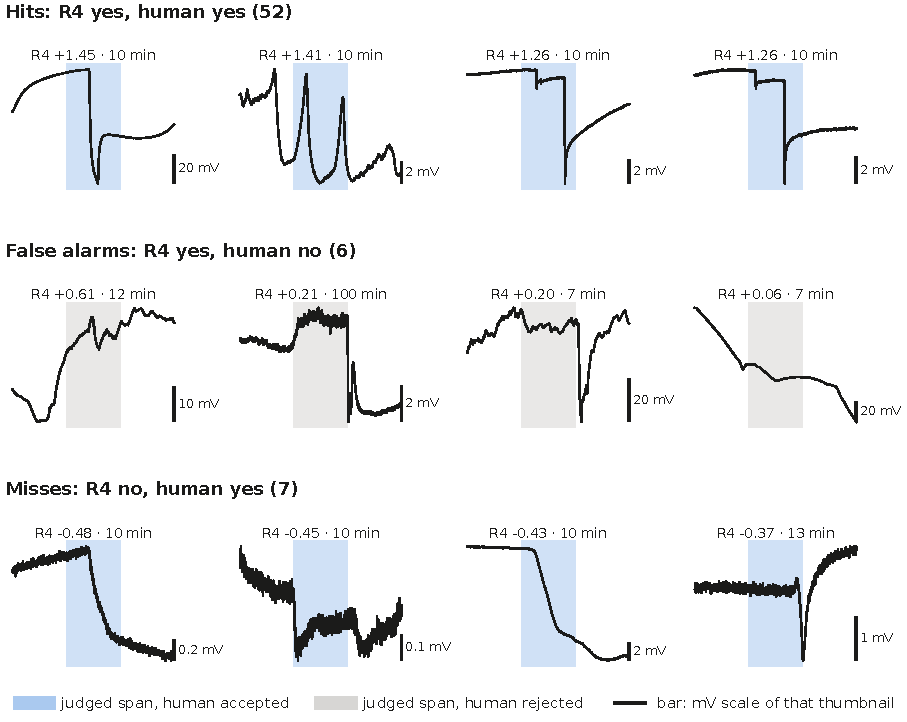
\includegraphics[width=\textwidth]{new/ch8_r4_examples.pdf}
\caption[{What R4 gets right and wrong on the original M4 classifier examination.}]{What R4 gets right and wrong on the original M4 classifier examination, at its pre-specified threshold: among 257 scored cases, 52 hits, six false alarms, seven misses and 192 correct rejections. Rows show the most confident hits (R4 yes, human yes), the most confident false alarms (R4 yes, human no) and the clearest misses (R4 no, human yes). Each judged span is shaded by the human verdict (blue accepted, grey rejected) and shown with its own length of context either side; each panel has its own millivolt scale bar, with R4's decision value and the span's duration above it. Two of the false alarms hold a sharp fall at or just beyond the edge of the judged span, and two of the misses are falls of only a fraction of a millivolt: the model and the reviewer part company at the edges of spans and at the smallest events.}
\label{fig:r4examples}
\end{figure}

\begin{figure}[htbp]
\centering
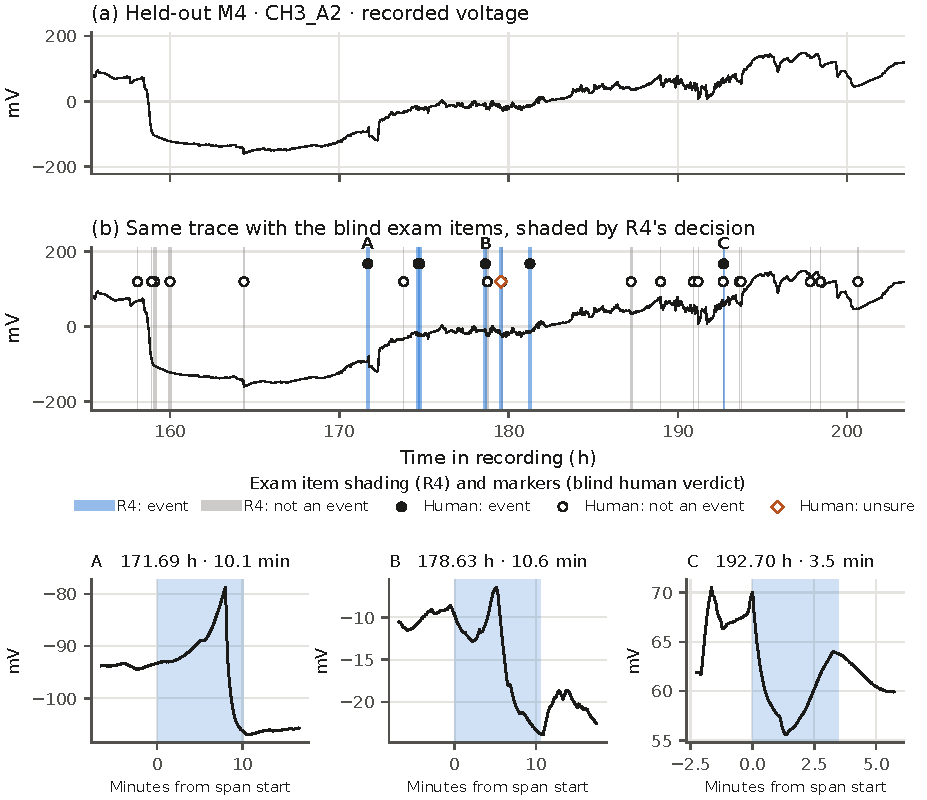
\includegraphics[width=\textwidth]{new/ch8_m4_before_after.pdf}
\caption[{The held-out recording before and after scoring.}]{The held-out recording before and after scoring. (a) A 48-hour excerpt of M4 CH3\_A2 (155.4--203.4 hours). (b) The same trace with the 25 exam items that fall in it: each judged span is shaded blue where the frozen R4 calls it an event and grey where it does not, and the markers give the blind verdict (filled, upper row: accepted; open, lower row: rejected; diamond: unsure). R4 agrees with the human verdict on all 24 answered items here; the one unsure item is one R4 calls an event. A--C zoom in on three items that were both accepted and called events by R4, at their original voltage and time scales (10.1, 10.6 and 3.5 minutes long), with the judged span shaded. Exam-wide performance is in Table~\ref{tab:exam}.}
\label{fig:m4beforeafter}
\end{figure}

\clearpage

\section*{From Chapter~\ref{ch:events}: events}

\begin{figure}[htbp]
\centering
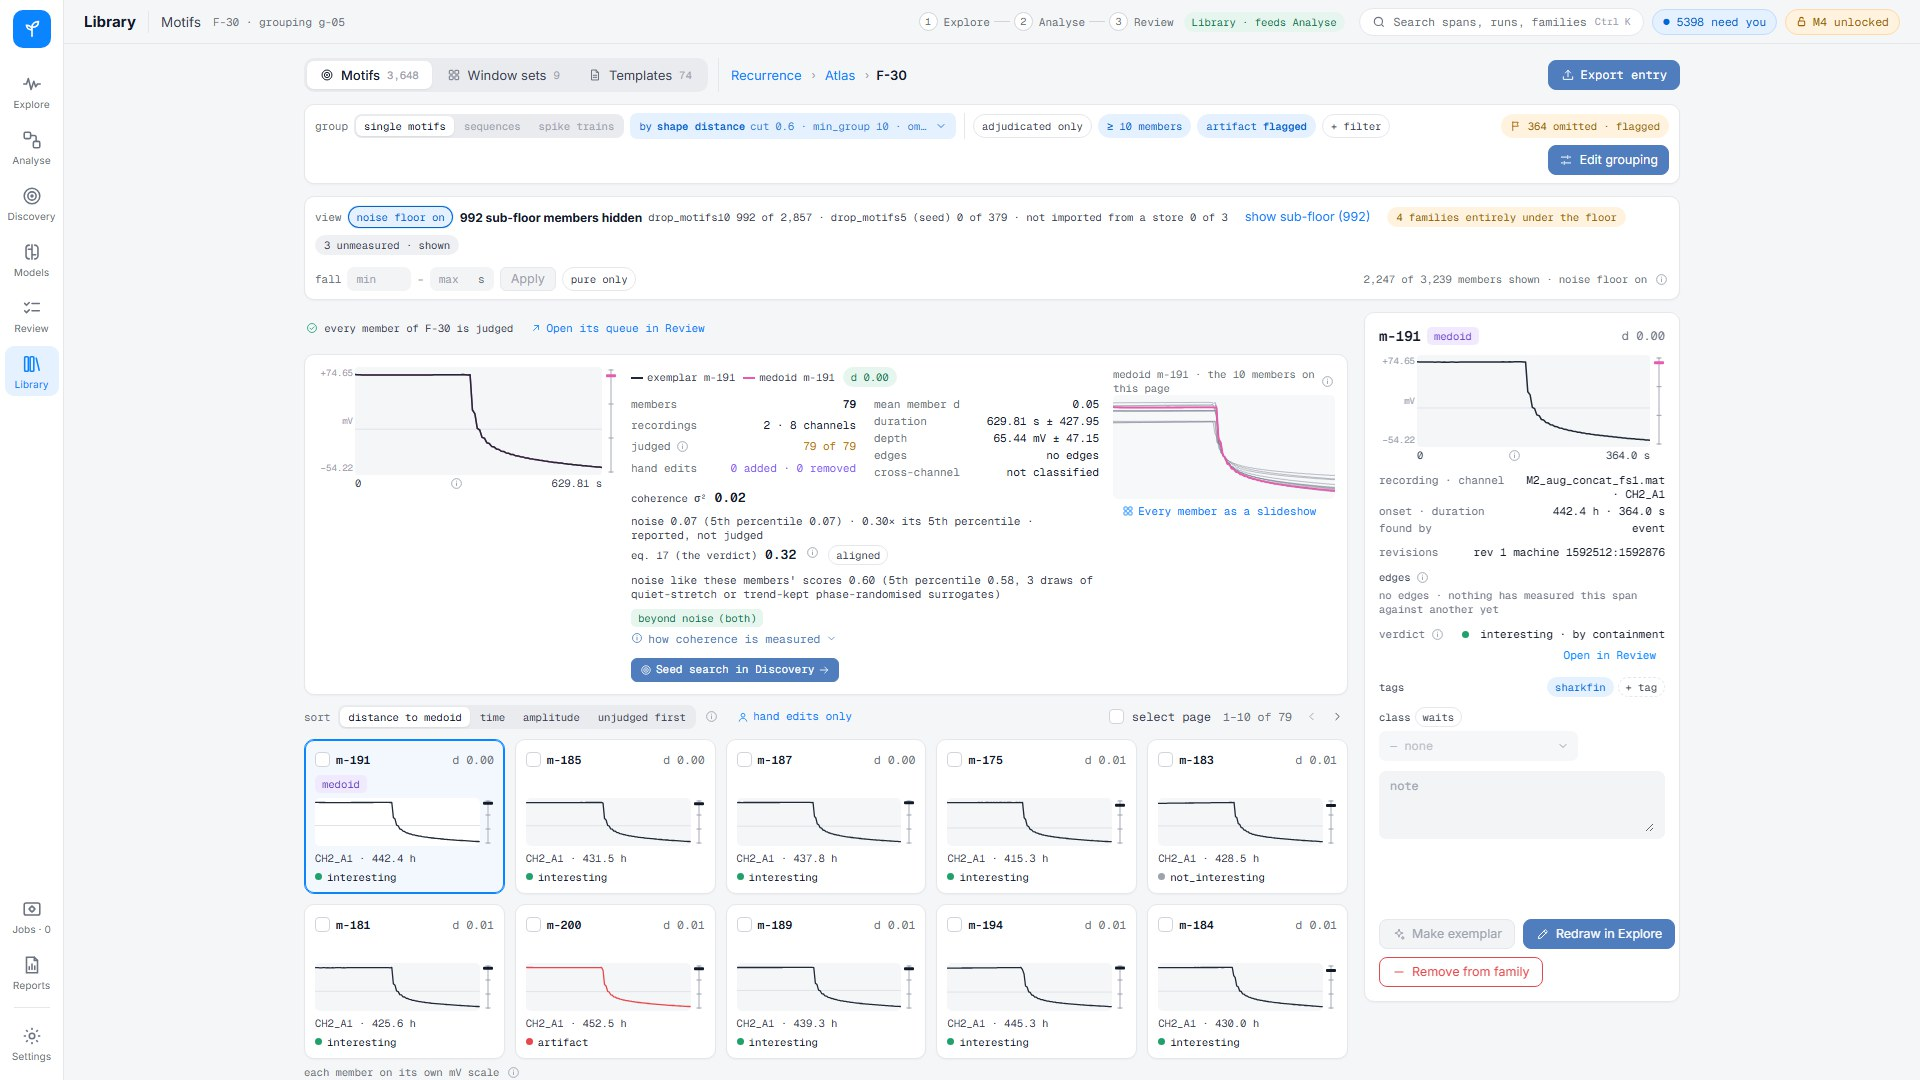
\includegraphics[width=\textwidth]{screens/library_family_f30.jpg}
\caption[{One Library family as the site shows it (F-30, grouping g-05).}]{One Library family as the site shows it (F-30, grouping g-05): 79 members drawn around their medoid. All 79 have been judged, and most were accepted; one was judged not interesting and one an artefact.}
\label{fig:familyf30}
\end{figure}

\begin{figure}[htbp]
\centering
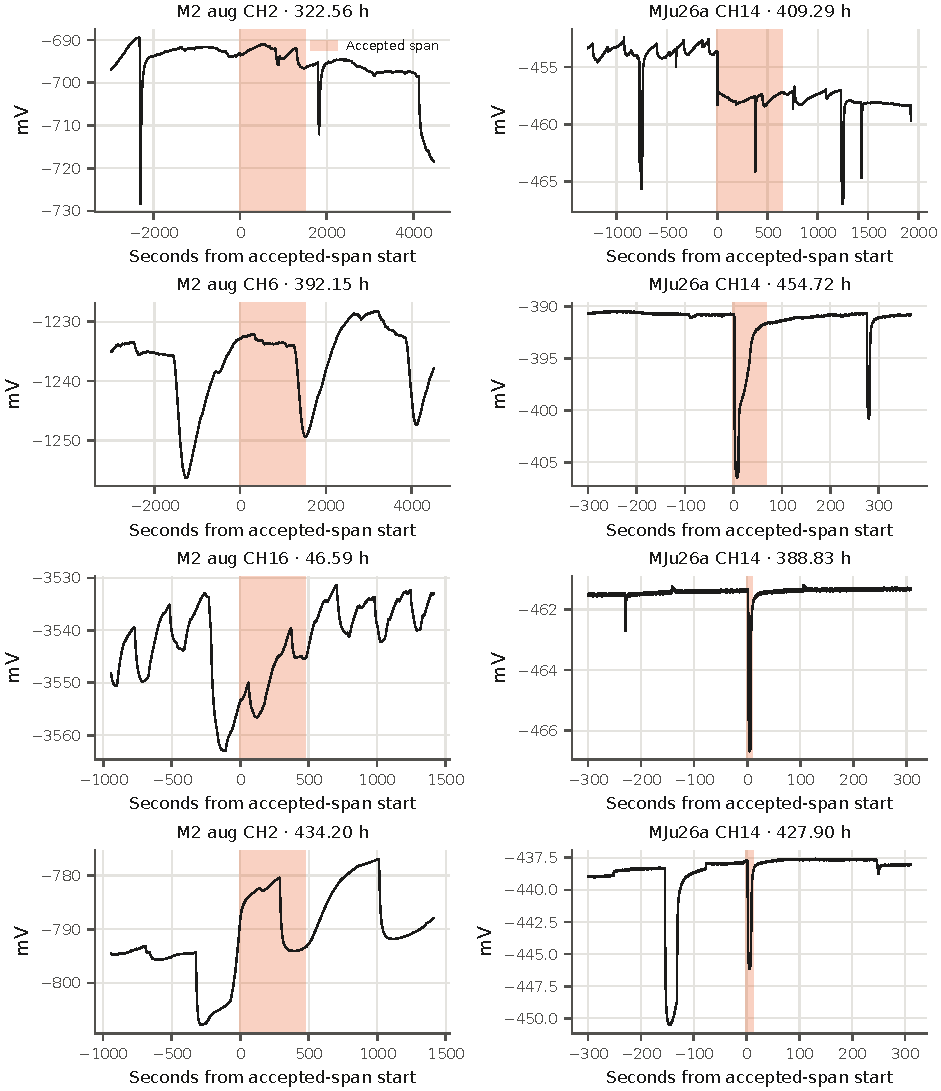
\includegraphics[width=\textwidth]{new/ch9_context_examples.pdf}
\caption[{Why an accepted span needs its surrounding signal.}]{Why an accepted span needs its surrounding signal. Left: newly reviewed Library proposals; right: spans from the long MJu26a CH14 train. Orange shading marks the accepted span; the black trace adds the signal either side, each panel on its own millivolt scale, with seconds measured from the span's start. An accepted span can hold only a small part of a deflection, only a recovery, or several adjacent shapes. The examples were chosen to show these boundary problems and are not a random sample of the catalogue.}
\label{fig:cataloguecontext}
\end{figure}

\begin{figure}[htbp]
\centering
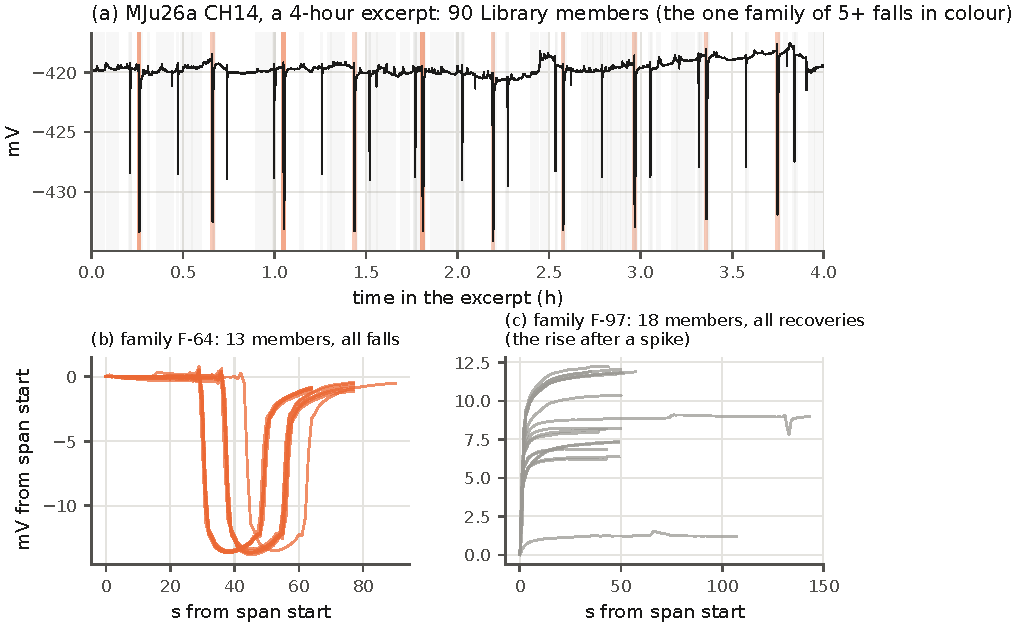
\includegraphics[width=\textwidth]{new/ch9_rec385.pdf}
\caption[{One recording in detail.}]{One recording in detail. (a) The 4-hour excerpt of MJu26a CH14 with its 90 Library members shaded; F-64, the one shape family here with five or more members that are falls, is in orange. (b) F-64's 13 members overlaid from the start of their spans (the falls come 30--55\,s in): the same fall recurs throughout the four hours. (c) The largest family, F-97 (18 members), drawn the same way: every member is the rise that follows a spike, not the spike itself, a reminder that a Library span can capture only part of a waveform (Section~\ref{sec:catalogue}). The two panels have their own voltage scales. Most other members sit in families of two or three.}
\label{fig:rec385}
\end{figure}

\begin{figure}[htbp]
\centering
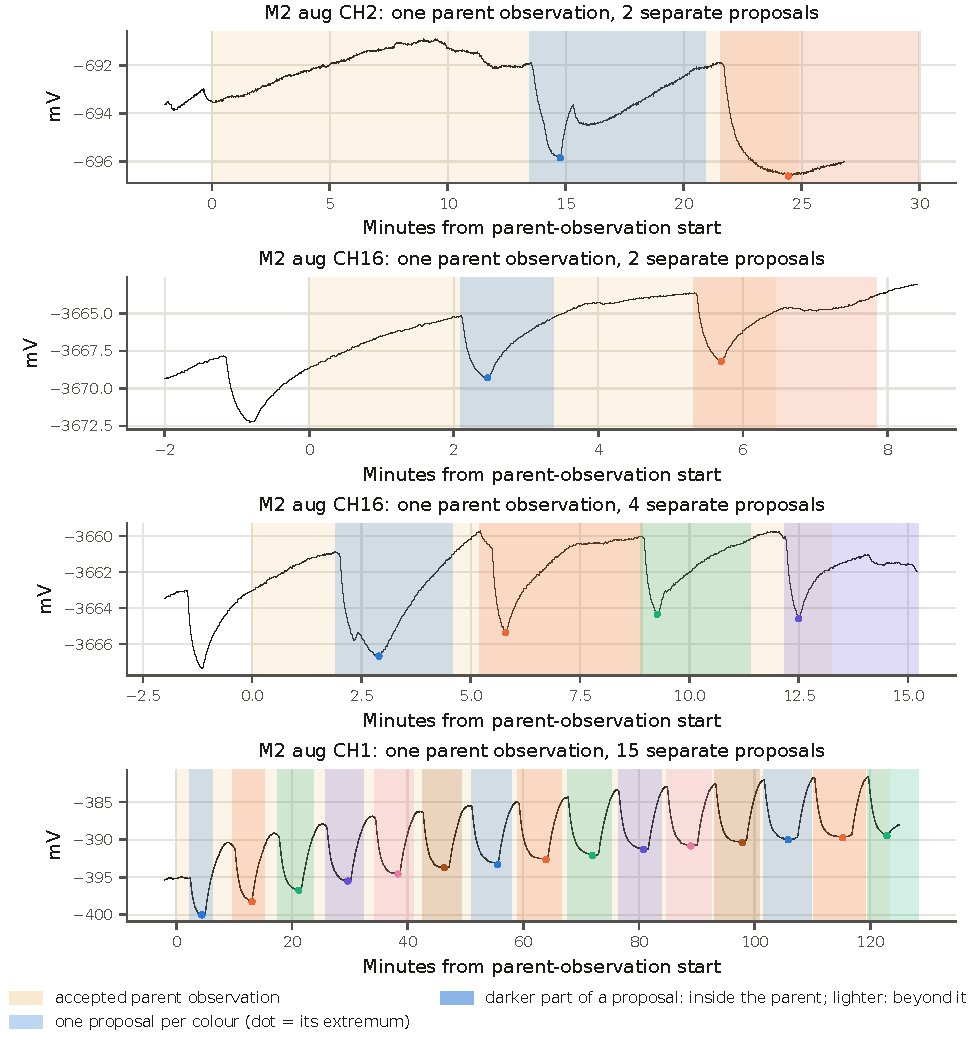
\includegraphics[width=\textwidth]{new/ch9_event_sequence_hierarchy.pdf}
\caption[{One accepted span and the individual events proposed inside it.}]{One accepted span and the individual events proposed inside it, for four spans ranging from a pair of events to a longer train. Pale orange shading marks the accepted span. Each proposed event has its own colour (colours only tell neighbours apart, not shape families) and a dot at its trough; the darker part of a proposal lies inside the accepted span and the lighter part runs beyond it. Each proposal runs from the shoulder before its fall to a return through 95\,\% of the fall, or to the start of the next event if that comes first, so neighbouring events stay separate. The proposals are unchecked.}
\label{fig:eventhierarchy}
\end{figure}

\begin{figure}[htbp]
\centering
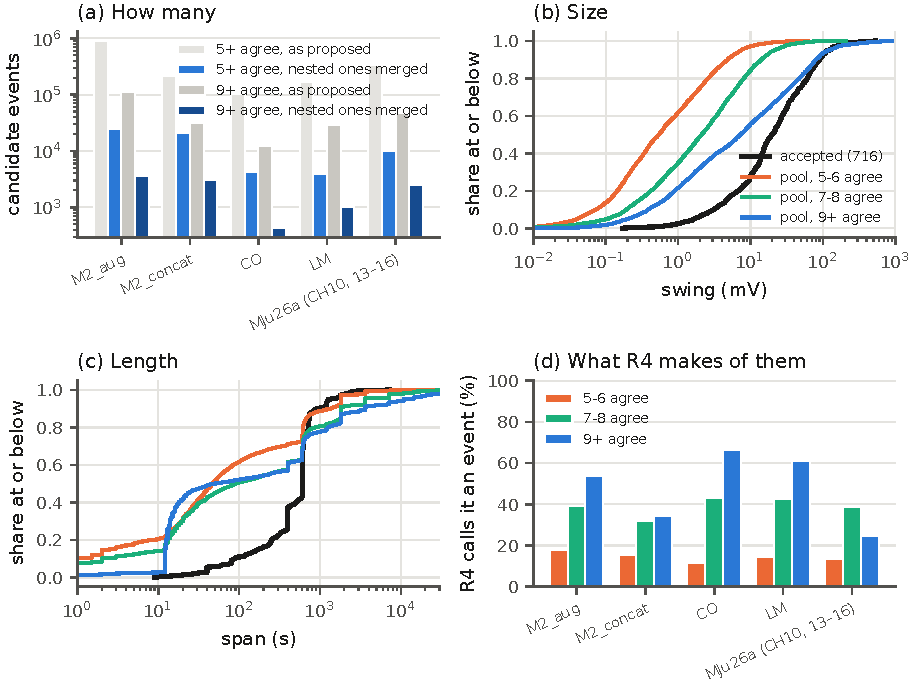
\includegraphics[width=\textwidth]{new/ch9_pool.pdf}
\caption[{Events no one has judged.}]{Events no one has judged. (a) Candidates on which five or more, and nine or more, detector families agree, as proposed and after merging nested ones (log scale). (b, c) The size and length of a stratified sample of 2,000 merged candidates per recording, by agreement, against the 716 accepted events (cumulative shares). (d) The share the frozen R4 classifier calls an event, by agreement.}
\label{fig:pool}
\end{figure}

\begin{figure}[htbp]
\centering
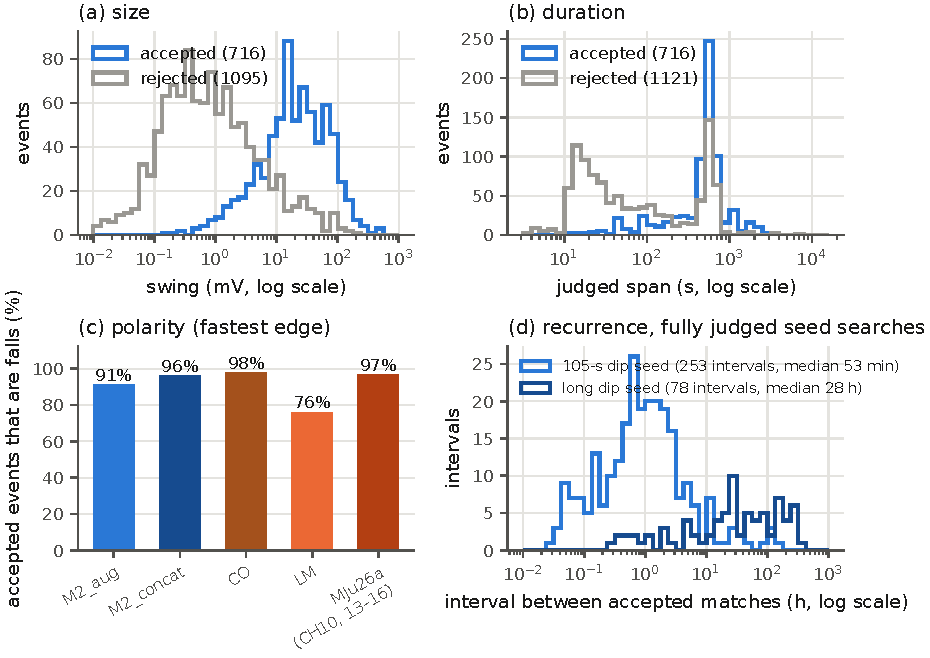
\includegraphics[width=\textwidth]{new/ch9_catalogue.pdf}
\caption[{The judged events of the two blind detector panels (five recordings).}]{The judged events of the two blind detector panels (five recordings). (a) Swing and (b) judged span length, accepted against rejected: accepted events are larger, and many spans are about 600\,s because detectors frame them that way. (c) The share of accepted events whose fastest edge is a fall, per recording. (d) Intervals between accepted matches on one channel, for the two seed searches judged in full (the short and long dips of Chapter~\ref{ch:rq2}).}
\label{fig:catalogue}
\end{figure}

\begin{figure}[htbp]
\centering
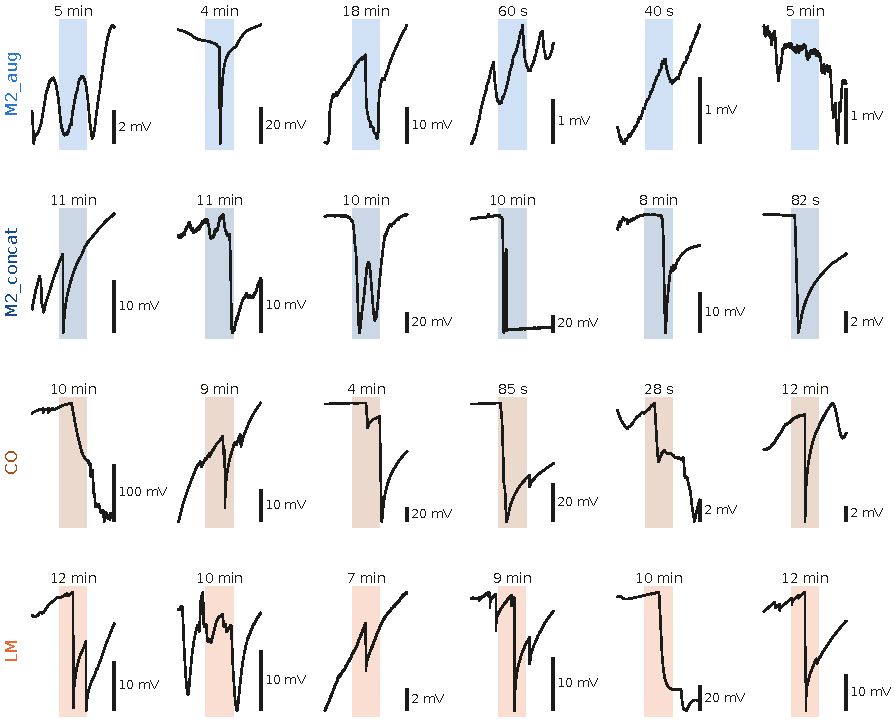
\includegraphics[width=\textwidth]{new/ch9_accepted_gallery.pdf}
\caption[{What an accepted event looks like.}]{What an accepted event looks like: six accepted events from each of four recordings, drawn at random, each shaded and shown with its own length of context either side. Each panel has its own scale; the bar gives millivolts and the title the event's length. Most are falls in potential, from seconds to tens of minutes long and from a few to a hundred millivolts deep, and many hold more than one deflection.}
\label{fig:acceptedgallery}
\end{figure}

\clearpage

\section*{From Chapter~\ref{ch:roundb}: the signal studies}

\begin{table}[htbp]
\caption[{The questions studied in this chapter.}]{The questions studied in this chapter: the site page that answers each, its data, its null, and the building it needed. B7 (multiscale entropy) and B8 (motif prevalence) were not run; they are future work (Section~\ref{sec:futurework}).}
\label{tab:roundb}
\footnotesize
\begin{tabularx}{\textwidth}{@{}l >{\raggedright\arraybackslash}X >{\raggedright\arraybackslash}p{3.1cm} >{\raggedright\arraybackslash}p{2.5cm} >{\raggedright\arraybackslash}p{2.3cm} >{\raggedright\arraybackslash}p{1.5cm}@{}}
\toprule
\textbf{\#} & \textbf{Question} & \textbf{On the site} & \textbf{Data} & \textbf{Null} & \textbf{Build}\\
\midrule
B1 & Are the intervals between events regular, bursty or random? & Interrogation $\rightarrow$ Intervals (LV, CV2) & drop-detector events, active sets & random timing; shuffled intervals & small\\
B2 & Do drop sequences change shape step by step more than chance? & Library $\rightarrow$ Sequences, on g-11 & M2\_aug, M2\_concat, CO, LM & shuffled order & small\\
B3 & Does a drop's recovery depend on the gap before it? & Event shape and Intervals (restitution) & sequences and chains; the drop-detector census & shuffled gaps & backend\\
B4 & Is cross-channel activity propagation or a shared-ground artefact? (plan RQ6) & Explore $\rightarrow$ Cross-channel (the explorer, S0--S1 at least) & the seven sets & rotation; random time & explorer build\\
B5 & What do the Discovery Maps show about when and where detectors fire? & Discovery $\rightarrow$ Map & all swept sets & paired surrogate runs; time-shifted rates & none\\
B6 & Do the same shape families occur across recordings and species? & Library $\rightarrow$ Atlas, Recurrence, on g-11 & M2\_aug, M2\_concat, CO, LM & shuffled recording labels & none\\
B9 & Do event durations cluster at preferred scales? & \texttt{cwt\_events} & all swept sets & AAFT surrogates & none\\
B10 & At which time scales does structure beyond noise appear? & \texttt{motif\_lengths}; CNN templates at 1, 10, 60\,min; \texttt{spike\_event\_\allowbreak features} & M2\_aug, M2\_concat, CO, LM, MJu26a & AAFT surrogates & none\\
B11 & Do the detectors find the same events on the newer datasets? & Discovery $\rightarrow$ Compare; Compare every stage & CO, LM, MJu26a, SH, SO & per-run surrogate & none\\
B12 & Do spike and drop shapes and intervals differ between recordings and species? & Interrogation $\rightarrow$ Event shape, Intervals, on accepted events & M2\_aug, M2\_concat, CO, LM & shuffled recording labels & none\\
\bottomrule
\end{tabularx}
\end{table}

\begin{figure}[htbp]
\centering
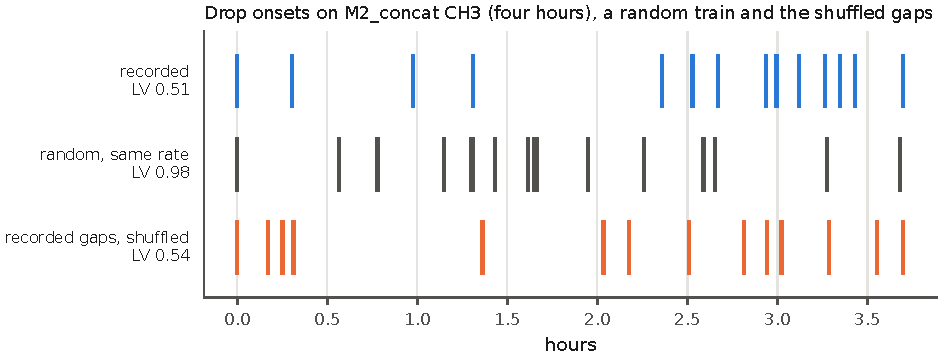
\includegraphics[width=\textwidth]{new/ch10_b1_train.pdf}
\caption[{B1 in the signal: drop onsets on four hours of M2\_concat CH3.}]{B1 in the signal: the drop onsets of four hours of M2\_concat CH3 (top; the train of Figure~\ref{fig:anatomytrain}), a random (Poisson) train at the same rate (middle), and the recorded gaps in a shuffled order (bottom), each with its LV. The recorded train (LV 0.51) is more regular than the random one (0.98), and a little more regular than its own gaps shuffled (0.54): a few short gaps cluster together near the end of the four hours, the kind of pattern a slowly changing rate produces. This window was chosen for having the most drops, and is one of the more regular stretches; across whole channels, most trains sit closer to the random row (Figure~\ref{fig:b1lv}).}
\label{fig:b1train}
\end{figure}

\begin{figure}[htbp]
\centering
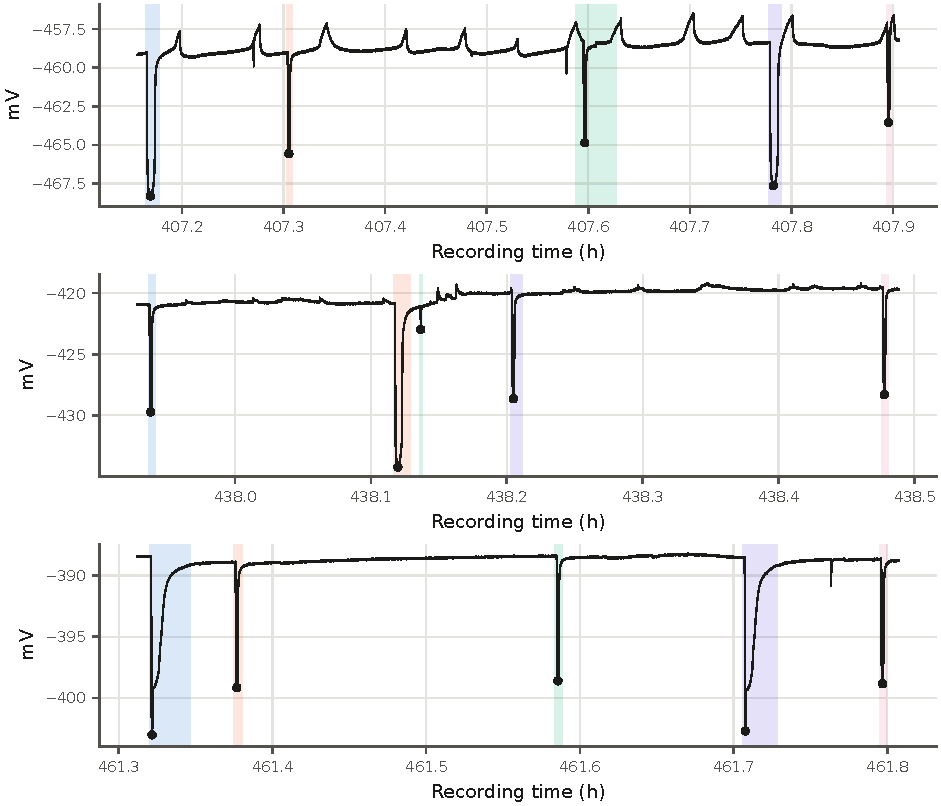
\includegraphics[width=\textwidth]{new/ch10_ch14_separate_events.pdf}
\caption[{Individual spikes within the CH14 train.}]{Individual spikes within the CH14 train: five consecutive spikes from the middle of each third of the train, in their surrounding signal. Black dots mark each spike's trough; colours only tell neighbouring spikes apart. Each spike's extent ends where the next spike begins, so a following spike is never absorbed into the tail of the one before. Uncoloured deflections are simply outside the five shown. The extents are machine proposals inside accepted spans, still to be checked by hand.}
\label{fig:ch14individuals}
\end{figure}

\begin{table}[htbp]
\centering\small
\caption[{How the CH14 train's timing results depend on the smallest spike counted.}]{How the CH14 train's timing results depend on the smallest spike counted (the prominence floor), with the 0.5\,s smoothing and 3\,s minimum separation held fixed. Only troughs inside accepted spans are counted; both nulls use 1,000 draws. The train was chosen by eye, so these are tests of a selected train, not of the whole recording.}
\label{tab:ch14sensitivity}
\begin{tabular}{@{}rrrrr@{}}
\toprule
\makecell[r]{\textbf{Prominence}\\\textbf{floor (mV)}} & \makecell[r]{\textbf{Supported}\\\textbf{extrema}} & \textbf{LV} & \makecell[r]{\textbf{Random timing}\\\boldmath$p$} & \makecell[r]{\textbf{Shuffled gaps}\\\boldmath$p$}\\
\midrule
0.5 & 542 & 0.712 & 0.002 & 0.002\\
1.0 & 530 & 0.708 & 0.002 & 0.006\\
2.0 & 503 & 0.682 & 0.002 & 0.885\\
\bottomrule
\end{tabular}
\end{table}

\begin{figure}[htbp]
\centering
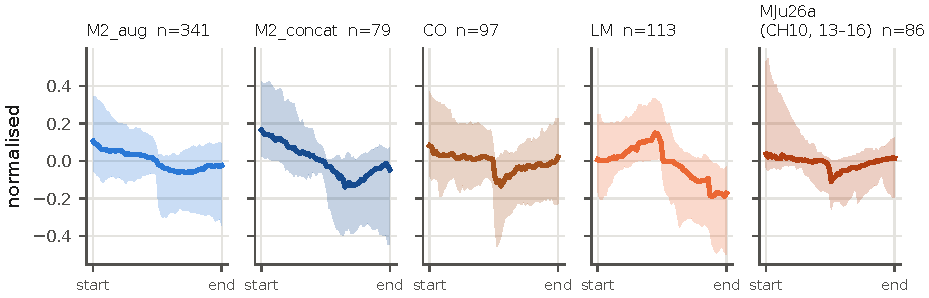
\includegraphics[width=\textwidth]{new/ch10_b12_waveforms.pdf}
\caption[{B12 in the signal: accepted events stretched to a common length.}]{B12 in the signal: each recording's accepted events stretched to a common length (start to end of the judged span). Each event is normalised by subtracting its median and dividing by its range, so every event spans one unit; the line is the median across events and the band the middle half. Every recording's typical event is a fall, placed at different points in its span; the shapes differ in detail, and LM's events more often begin with a rise.}
\label{fig:b12waves}
\end{figure}

\begin{figure}[htbp]
\centering
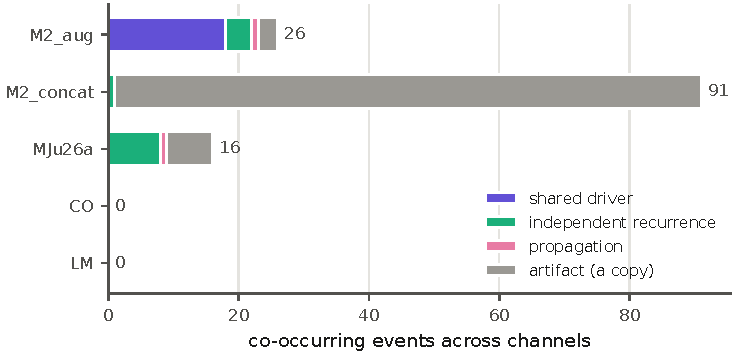
\includegraphics[width=0.85\textwidth]{new/ch10_b4_bins.pdf}
\caption[{The B4 census: drop-detector events on several channels at once.}]{The B4 census: \texttt{drop\_detection\_v1} events that occur on two or more channels together, per recording, by what the census classifies them as. These are per-event classifications, not tests; the tests against rotation and random-time nulls are in the text. M2\_concat's are copies between channels; CO and LM have none.}
\label{fig:b4bins}
\end{figure}

\begin{figure}[htbp]
\centering
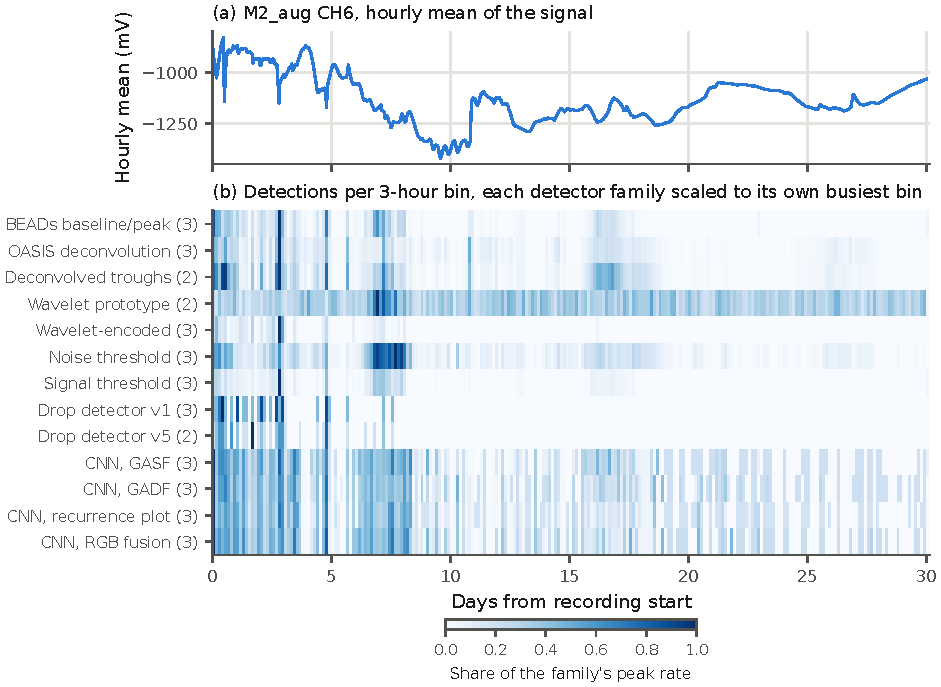
\includegraphics[width=\textwidth]{new/ch10_b5_timeline.pdf}
\caption[{B5 on one channel, M2\_aug CH6, redrawn from the Discovery Map's own counts.}]{B5 on one channel, M2\_aug CH6, redrawn from the Discovery Map's own counts. (a) The signal's hourly mean over the 30 days. (b) Detections in 3-hour bins for 13 detector families (number of settings in brackets), each row scaled to its own busiest bin. Families that look for very different things are busiest together, in the first eight days and again around days 15--17, and quieter in between and after; the drop detectors fire only in the first eight days. The paired phase-randomised copies do not rise and fall like this, so the pattern is the recording's own activity changing over days.}
\label{fig:b5timeline}
\end{figure}

\begin{figure}[htbp]
\centering
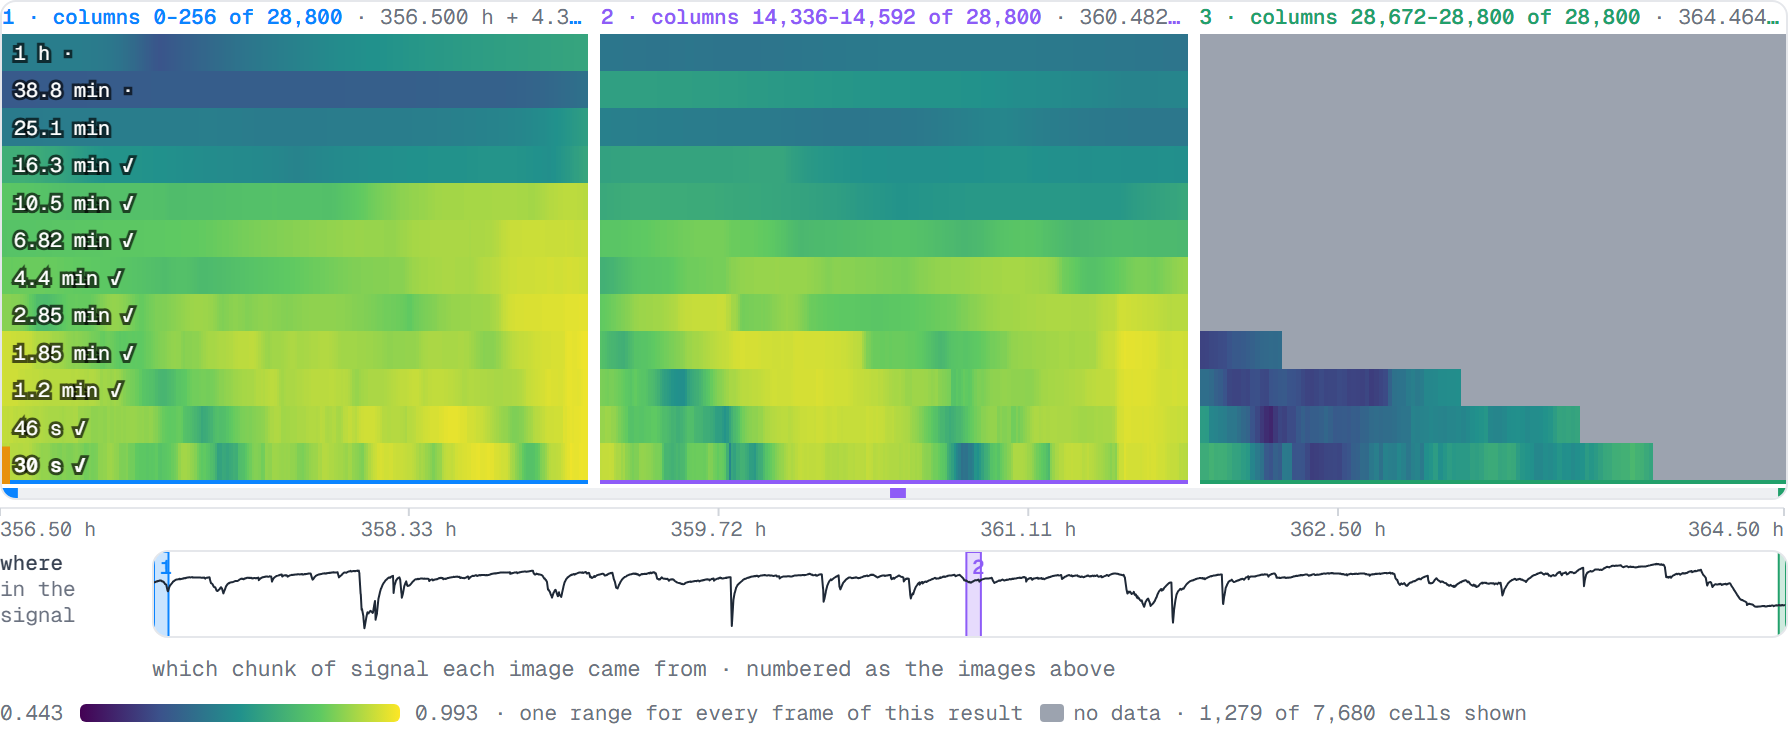
\includegraphics[width=\textwidth,height=0.55\textheight,keepaspectratio]{roundb/b10_motif_lengths_m2aug_crop.png}
\caption[{B10 on the site: \texttt{motif\_lengths} on eight hours of M2\_aug.}]{B10 on the site: \texttt{motif\_lengths} on eight hours of M2\_aug (356.5--364.5\,h). Each image is one chunk of the pan matrix profile, from the start, middle and end of the span (located on the signal strip beneath); each row is a window length, from 30\,s at the bottom to one hour at the top, and the colour is each window's distance to its nearest match elsewhere in the span (darker is a closer repeat). A tick marks a length whose repeats are closer than in the AAFT copies of the same span: every length from 30\,s to 16.3\,min, with no single length standing out. The two longest lengths cannot be judged on eight hours.}
\label{fig:b10motif}
\end{figure}

\begin{figure}[htbp]
\centering
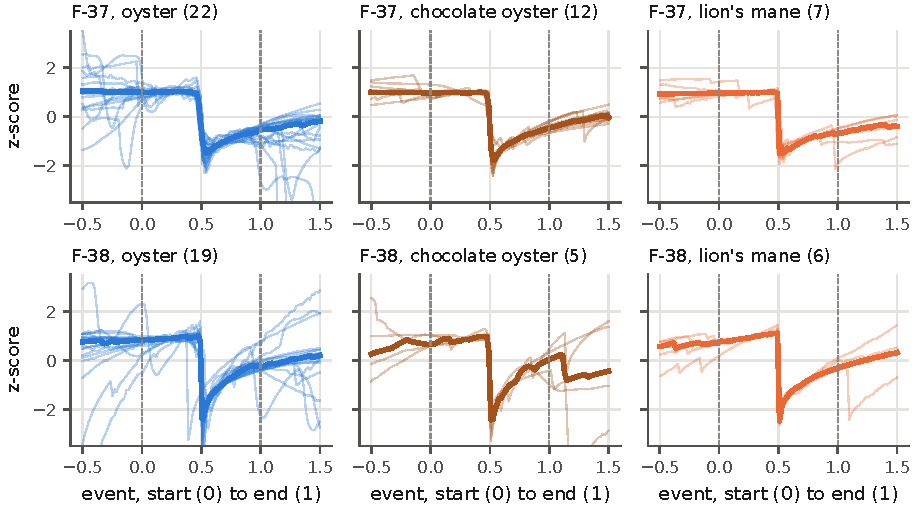
\includegraphics[width=\textwidth]{new/ch10_b6_species.pdf}
\caption[{B6 in the signal: two g-11 families shared by three cultures.}]{B6 in the signal: the two g-11 families with at least four members on each of three cultures, oyster and chocolate oyster (two strains of \emph{P.\ ostreatus}) and lion's mane (\emph{H.\ erinaceus}). Each member is z-normalised and stretched so its event runs from 0 to 1 (dashed lines), with half its length of context either side; the bold line is the median. The same sudden fall and slow recovery appears in both species.}
\label{fig:b6species}
\end{figure}

\begin{table}[htbp]
\centering
\caption[{The completed 2\,Hz sweep: detections on the recordings and their copies.}]{The completed 2\,Hz sweep: detections on each recording and on its phase-randomised copy (recording/copy), by detector family, summed over the family's settings (in brackets) and over 16 channels for MJu26a and four each for SH and SO. Each channel has one copy. The first group found more on the recording on all three, the second on some, and the third found more on the copy on all three. These are detection counts, not grouped or human-accepted events.}
\label{tab:rq4partialreturns}
\small
\begin{tabularx}{\textwidth}{@{}Xrrr@{}}
\toprule
\textbf{Family (settings)} & \textbf{MJu26a} & \textbf{SH} & \textbf{SO}\\
\midrule
Deconvolved troughs (3) & 414,921/4,526 & 119,583/957 & 103,298/922\\
OASIS (3) & 358,284/7,175 & 53,380/1,218 & 70,066/1,211\\
Matrix-profile threshold (1) & 62,527/7,248 & 22,148/6,015 & 80,053/10,042\\
Noise threshold (3) & 31,376/1,023 & 7,407/226 & 8,260/199\\
CNN, 60\,min (4) & 4,948/3,964 & 1,263/695 & 1,250/607\\
Drop v1 (3) & 1,529/460 & 58/36 & 75/27\\
\midrule
Drop v5 (3) & 2,466/3,717 & 72/16 & 129/9\\
CNN, 10\,min (4) & 26,648/22,377 & 2,993/3,444 & 2,394/3,014\\
\midrule
Wavelet prototype (3) & 167,199/214,236 & 27,632/38,601 & 23,185/37,972\\
Symbol search (3) & 111,312/443,710 & 1,808/85,295 & 17,244/86,093\\
BEADs (3) & 2,439/25,118 & 1,135/12,599 & 574/6,918\\
Signal threshold (3) & 3,911/116,630 & 3,635/76,986 & 1,519/37,931\\
Wavelet encoded (3) & 5,072/117,050 & 104/21,962 & 172/22,011\\
CNN, 1\,min (4; negative control) & 226,525/467,918 & 17,618/99,610 & 10,446/81,817\\
\bottomrule
\end{tabularx}
\end{table}

\begin{figure}[htbp]
\centering
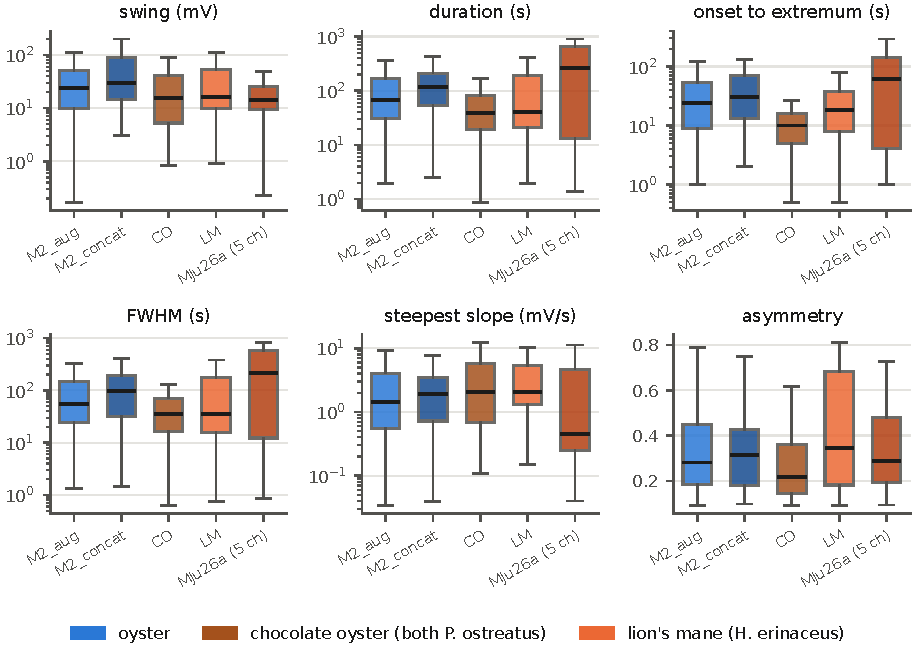
\includegraphics[width=\textwidth]{new/ch10_b12_shape.pdf}
\caption[{B12: six shape measures of the 716 accepted blind-queue events.}]{B12: six shape measures of the 716 accepted blind-queue events, by recording, coloured by species and strain (boxes are quartiles, whiskers the 5--95\,\% range). The recordings differ, but only a little, and two recordings of one species differ about as much as the species do.}
\label{fig:b12shape}
\end{figure}

\clearpage
